\documentclass{article}

\usepackage[utf8]{inputenc}
\usepackage{authblk}
\usepackage{setspace}
\usepackage[margin=1.25in]{geometry}
\usepackage{graphicx}
\graphicspath{{./figures/}}
\usepackage{subcaption}
\usepackage{amsmath}
\usepackage{amssymb}
\usepackage{booktabs}
\usepackage{longtable,pdflscape}
\usepackage[T1]{fontenc}
\usepackage{lmodern}
\input{glyphtounicode}
\pdfgentounicode=1
\usepackage{array}
\usepackage{tabularx}
\usepackage{lineno}
\usepackage[
  style=nejm,
  citestyle=numeric-comp,
  sorting=none
]{biblatex}
\addbibresource{references.bib}
\usepackage[hidelinks]{hyperref}
\hypersetup{
  pdftitle={Precision Synthesis of Multi-Tracer PET via VLM-Modulated Rectified Flow for MCI Stage Stratification},
  pdfauthor={Shuijin Lin; Shaozhen Yan; Tuo Liu; Haifeng Wang; Chunfeng Lian; Jie Lu; Jianhua Ma; Lin Xie},
  pdfsubject={Research Article},
  pdfkeywords={Controllable Cross-Modal Synthesis; Domain-Knowledge Encoding; PET Imaging; Alzheimer's Disease; Vision-Language Model; Rectified Flow}
}

\title{Precision Synthesis of Multi-Tracer PET via VLM-Modulated Rectified Flow for MCI Stage Stratification}

\author[1,4,$\dagger$]{Shuijin Lin}
\author[2,$\dagger$]{Shaozhen Yan}
\author[3,4,$\dagger$]{Tuo Liu}
\author[3,4]{Haifeng Wang}
\author[3,4]{Chunfeng Lian}
\author[2,*]{Jie Lu}
\author[1,4,*]{Jianhua Ma}
\author[1,4,*]{Lin Xie}

\affil[1]{Key Laboratory of Biomedical Information Engineering of Ministry of Education, School of Life Science and Technology, Xi'an Jiaotong University, No.~28 Xianning West Road, Xi'an, Shaanxi 710049, China.}
\affil[2]{Department of Radiology and Nuclear Medicine, Xuanwu Hospital, Capital Medical University, No.~45 Changchun Street, Xicheng District, Beijing 100053, China.}
\affil[3]{School of Mathematics and Statistics, Xi'an Jiaotong University, No.~28 Xianning West Road, Xi'an, Shaanxi 710049, China.}
\affil[4]{Research Center for Intelligent Medical Equipment and Devices (IMED), Xi'an Jiaotong University, No.~28 Xianning West Road, Xi'an, Shaanxi 710049, China.}
\affil[*]{Address correspondence to: Jie Lu, \href{mailto:imaginglu@hotmail.com}{imaginglu@hotmail.com}; Jianhua Ma, \href{mailto:jhma@xjtu.edu.cn}{jhma@xjtu.edu.cn}; Lin Xie, \href{mailto:linxie@xjtu.edu.cn}{linxie@xjtu.edu.cn}.}
\affil[$\dagger$]{These authors contributed equally to this work.}

\date{}

\emergencystretch=2em
\onehalfspacing
\linenumbers

\newlabel{fig:supp_av45_1}{{S1}{25}{\textbf {Comparison of real and synthetic AV45 uptake across the remaining brain regions (Part 1 of 2).} Values represent mean regional intensities from per-image min--max-normalized PET images (arbitrary units), rather than SUVR.\relax }{figure.caption.15}{}}
\newlabel{fig:supp_av45_2}{{S2}{26}{\textbf {Comparison of real and synthetic AV45 uptake across the remaining brain regions (Part 2 of 2).} Values represent mean regional intensities from per-image min--max-normalized PET images (arbitrary units), rather than SUVR.\relax }{figure.caption.16}{}}
\newlabel{fig:supp_fdg_1}{{S3}{27}{\textbf {Comparison of real and synthetic FDG uptake across the remaining brain regions (Part 1 of 2).} Values represent mean regional intensities from per-image min--max-normalized PET images (arbitrary units), rather than SUVR.\relax }{figure.caption.17}{}}
\newlabel{fig:supp_fdg_2}{{S4}{28}{\textbf {Comparison of real and synthetic FDG uptake across the remaining brain regions (Part 2 of 2).} Values represent mean regional intensities from per-image min--max-normalized PET images (arbitrary units), rather than SUVR.\relax }{figure.caption.18}{}}
\newlabel{fig:supp_disease_av45}{{S5}{29}{\textbf {Validation of disease-related AV45 uptake patterns across the remaining brain regions.} Violin plots display mean normalized regional uptake (arbitrary units) in Alzheimer’s disease (AD, red) and cognitively normal (CN, green) subjects for selected brain regions. Each region contains paired half-violins: the left half (solid fill) represents real PET data, and the right half (dashed fill) represents MRI-synthetic PET data, with consistent color coding between modalities. Solid lines above the violins indicate statistical significance for real PET, while dashed lines indicate significance for synthetic PET. Uptake values were derived from per-image min--max-normalized PET images without reference-region normalization.\relax }{figure.caption.19}{}}
\newlabel{fig:supp_disease_fdg}{{S6}{30}{\textbf {Validation of disease-related FDG uptake patterns across the remaining brain regions.} Violin plots display mean normalized regional uptake (arbitrary units) in Alzheimer’s disease (AD, red) and cognitively normal (CN, green) subjects for selected brain regions. Each region contains paired half-violins: the left half (solid fill) represents real PET data, and the right half (dashed fill) represents MRI-synthetic PET data, with consistent color coding between modalities. Solid lines above the violins indicate statistical significance for real PET, while dashed lines indicate significance for synthetic PET. Uptake values were derived from per-image min--max-normalized PET images without reference-region normalization.\relax }{figure.caption.20}{}}
\newlabel{tab:supp_adni}{{S1}{31}{\textbf {Demographic characteristics and prepared clinical inputs of ADNI.} Data are mean $\pm $ sample s.d., except counts. Demographic $P$ values use one-way ANOVA (age, weight) or a chi-square test (sex). Clinical summaries combine observed and diagnostic-group-conditioned filled scores; their group-comparison $P$ values are omitted because the distributions are not independent clinical evidence. Source missingness is reported in Table~\ref {tab:clinical_missingness}. CDR: Clinical Dementia Rating; MMSE: Mini-Mental State Examination.\relax }{table.caption.21}{}}
\newlabel{tab:supp_oasis}{{S2}{31}{\textbf {Demographic characteristics of OASIS-3.}\relax }{table.caption.22}{}}
\newlabel{tab:supp_software}{{S3}{32}{\textbf {Historical core software dependencies and reported versions for DIReCT$++$.} This retained environment list describes the historical configuration; reconstructed training and the timing run used separately recorded environments. In particular, the RTX 4090 timing run used PyTorch 2.5.1+cu121, as stated in Methods. The table is not a single environment specification for every experiment.\relax }{table.caption.23}{}}
\newlabel{tab:clinical_missingness}{{S4}{32}{\textbf {Missing clinical scores in the source records before historical filling.} Each cell gives missing count / group size (percentage); missingness is defined relative to the first source CSV record selected for each participant, not all ADNI visits.\relax }{table.caption.24}{}}
\newlabel{tab:reproducibility}{{S5}{33}{\textbf {Reproducibility settings and scope of the revised analyses.}\relax }{table.caption.25}{}}
\newlabel{tab:supp_tau_adapter}{{S6}{34}{\textbf {Adapter-level sensitivity analysis of the cross-tracer soft target.} Descriptive means across two folds, using 1,856 QC-filtered participants. Only training-fold PET features were used for fitting; held-out features were evaluated after optimization. No cross-term means removal of the penalty ($\lambda _{\mathrm {cross}}=0$), not a target of zero. No generator was retrained or evaluated in this analysis.\relax }{table.caption.27}{}}
\newlabel{tab:regional_agreement}{{S7}{35}{\textbf {Regional normalized uptake agreement and descriptive regression for the 16 representative tracer--ROI combinations in Figure~\ref {fig:4}A,B.} Overall cohorts from the author-designated historical ROI CSVs; N can vary by ROI.\relax }{table.caption.28}{}}
\newlabel{tab:regional_effect_sizes}{{S8}{36}{\textbf {AD--CN regional effect sizes and BH-FDR-adjusted comparisons for Figure~\ref {fig:4}C--F.} Cohen's $d$ is AD minus CN divided by the pooled within-group sample s.d.\relax }{table.caption.29}{}}
\newlabel{tab:whole_volume_generation}{{S9}{37}{Whole-volume OOF generation metrics (mean $\pm $ sample s.d.)\relax }{table.S9}{}}
\newlabel{tab:paired_generation}{{S10}{38}{Paired whole-volume generation comparisons\relax }{table.S10}{}}
\newlabel{tab:r3_11_masked_summary}{{S11}{40}{Mask-restricted quality of frozen two-fold OOF PET predictions.\relax }{table.caption.30}{}}
\newlabel{tab:r3_11_masked_paired}{{S12}{40}{Paired mask-restricted PET image-quality comparisons.\relax }{table.caption.31}{}}
\newlabel{fig:cases_fdg}{{S7}{41}{\textbf {FDG synthesis in median, 10th-percentile and worst QC-passed cases.} Rows follow the frozen whole-volume SSIM selection; columns show MRI, real PET, synthetic PET and absolute-error maps. PET intensities and errors use the displayed [0,1] normalized-intensity scales. Selection is within the existing QC-passed set, without new exclusions or visual replacement; rankings use whole-volume SSIM rather than masked SSIM.\relax }{figure.caption.32}{}}
\newlabel{fig:cases_av45}{{S8}{42}{\textbf {AV45 synthesis in median, 10th-percentile and worst QC-passed cases.} Rows follow the frozen whole-volume SSIM selection; columns show MRI, real PET, synthetic PET and absolute-error maps. PET intensities and errors use the displayed [0,1] normalized-intensity scales. Selection is within the existing QC-passed set, without new exclusions or visual replacement; rankings use whole-volume SSIM rather than masked SSIM.\relax }{figure.caption.33}{}}
\newlabel{tab:classification_summary}{{S13}{43}{Three-fold classification results: mean $\pm $ sample s.d.; [conditional 95\% CI].\relax }{table.S13}{}}
\newlabel{tab:classification_comparisons}{{S14}{45}{Paired imaging classification differences\relax }{table.S14}{}}
\newlabel{tab:classification_clinical_comparisons}{{S15}{46}{Paired comparisons with clinical baselines\relax }{table.S15}{}}
\newlabel{tab:classification_delong}{{S16}{48}{Paired DeLong comparisons by outer fold\relax }{table.S16}{}}
\newlabel{fig:classification_roc}{{S9}{50}{\textbf {Cross-sectional classification ROC curves for AD/CN, EMCI+LMCI/CN and EMCI/LMCI (left to right).} Curves average three fold-specific TPRs at a fixed FPR grid; shaded regions are pointwise conditional 95\% bootstrap bands, not simultaneous confidence bands. Legend AUC values are equally weighted empirical fold AUC means. Comparisons include MRI, MRI+Real both, MRI+Syn both, Clinical-only and MRI+Clinical. The clinical fields include diagnosis-related scores and historical group-conditioned fills; high clinical AUC is not evidence of independent synthetic-PET benefit.\relax }{figure.caption.34}{}}
\newlabel{tab:e1_score_removal}{{S17}{50}{\textbf {E1 fixed-weight score-removal sensitivity.} Differences are No-Scores minus Full, except the nonnegative output difference between predictions. This is a distinct E1 Full checkpoint family, not the reconstructed Full used in the generator-comparison tables.\relax }{table.caption.35}{}}
\newlabel{tab:r2-16-ad-cn}{{S18}{51}{Age- and sex-stratified classification performance: AD vs CN.\relax }{table.caption.36}{}}
\newlabel{tab:r2-16-mci-cn}{{S19}{51}{Age- and sex-stratified classification performance: EMCI+LMCI vs CN.\relax }{table.caption.37}{}}
\newlabel{tab:r2-16-emci-lmci}{{S20}{51}{Age- and sex-stratified classification performance: EMCI vs LMCI.\relax }{table.caption.38}{}}

\begin{document}

\maketitle

\begin{abstract}
\noindent\textbf{Objective:} To evaluate DIReCT$++$, a domain-informed rectified flow framework for synthesizing FDG- and AV45-PET from MRI and clinical text inputs.

\noindent\textbf{Impact Statement:} This work evaluates multi-tracer synthesis and cross-sectional MCI stage discrimination, with explicit limits on clinical and prognostic interpretation.

\noindent\textbf{Introduction:} PET cost, radiation exposure and limited accessibility motivate MRI-based synthesis, but image similarity alone does not establish individual molecular validity.

\noindent\textbf{Methods:} A shared 3D rectified flow generator uses frozen BiomedCLIP-derived patient and tracer features for learned one-step inference. Separate analyses evaluate affine tracer adaptation, two-fold OOF generation, normalized regional uptake agreement and three-fold cross-sectional classification. ADNI includes 1,857 participants; historical OASIS-3 external evaluation is restricted to AV45 in CN/AD.

\noindent\textbf{Results:} Masked OOF comparisons favored Full over a clinical regression U-Net and MRI-only Swin-UNETR in all 16 predefined comparisons within their respective Holm families, although some effects were small. Other conditioning comparisons showed metric-dependent tradeoffs. In AD/CN classification, MRI+Syn-both AUC was $93.82\pm3.21\%$ versus MRI-only $87.02\pm5.44\%$; MCI/CN did not improve, and EMCI/LMCI showed mixed endpoints. Clinical-only and MRI+Clinical AUC exceeded MRI+Syn-both. Historical regional intensities showed close agreement, without establishing clinical SUV/SUVR calibration or equivalence.

\noindent\textbf{Conclusion:} DIReCT$++$ supports further investigation of multi-tracer synthesis and cross-sectional classification. Extensive diagnosis-conditioned filling of clinical scores, source-identity limitations and mixed task effects preclude claims of independent diagnostic value, longitudinal prognosis or replacement of molecular confirmation.
\end{abstract}

\noindent\textbf{Keywords:} Controllable Cross-Modal Synthesis; Domain-Knowledge Encoding; PET Imaging; Alzheimer's Disease; Vision-Language Model; Rectified Flow


\section{Introduction}
Alzheimer's disease (AD), the most prevalent neurodegenerative disorder, constitutes a mounting global health crisis. Its pathological processes begin years before clinical dementia manifests, making the prodromal stage of mild cognitive impairment (MCI) a critical window for intervention~\cite{scheltens2021alzheimer}. However, the heterogeneous nature of MCI, where only a subset of individuals progress to AD, poses a significant prognostic challenge~\cite{haller2023neuroimaging}. AD evaluation uses complementary molecular, functional and structural measurements: amyloid-$\beta$ (A$\beta$) deposition can be assessed with $^{18}$F-AV45 PET, glucose-metabolic dysfunction with $^{18}$F-FDG PET, and associated atrophy with structural MRI~\cite{ossenkoppele2022amyloid,yan2021sex,haller2023neuroimaging}. These modalities are not interchangeable; in particular, FDG hypometabolism and MRI atrophy do not by themselves establish the biological diagnosis of AD~\cite{jack2024revised}. In clinical practice, however, the routine acquisition of PET is hampered by high cost, limited access, and radiation exposure, limiting access to complementary imaging in research and selected diagnostic workups~\cite{nordberg2010use}.

Generative artificial intelligence (AI) offers a transformative pathway to bridge this clinical gap by synthesizing PET biomarkers from routinely acquired MRI~\cite{dayarathna2024deep,lee2024synthesizing}. Initial studies, primarily using generative adversarial networks (GANs)~\cite{pan2018synthesizing,pan2020spatially,apostolopoulos2022applications} and, more recently, diffusion models~\cite{xie2024synthesizing,chen2025multi,theodorou2025mri2pet}, have established the feasibility of producing visually realistic PET images. Subsequent advances have sought to improve fidelity by incorporating domain knowledge, for instance, through guidance from large vision-language models (VLMs)~\cite{wang2025unisyn,liu2025direct}.  Despite these advances, a critical limitation remains: the subject-specific precision necessary for cross-sectional diagnosis and MCI stage discrimination is still lacking, which is particularly crucial for a heterogeneous condition like AD~\cite{ossenkoppele2022amyloid}. This challenge stems from the inherent nature of MRI-to-PET synthesis as an ill-posed inverse problem; neurodegeneration visible on MRI is typically a downstream effect of prior molecular pathologies captured by PET~\cite{jagust2018imaging}. Consequently, individuals with similar structural MRI presentations at early disease stages can exhibit vastly different pathological burdens, leading to ambiguous mapping. Overcoming this ambiguity requires an AI synthesis framework that can comprehensively model complex cross-modal and cross-tracer associations to provide strong, patient-specific guidance.

Building upon single-tracer DIReCT~\cite{liu2025direct}, DIReCT$++$ (Domain-Informed ReCTified flow) extends 3D rectified flow to a shared network conditioned on the target PET tracer, enabling FDG- or AV45-PET generation in separate forward passes. A second extension is lightweight affine adaptation of BiomedCLIP~\cite{zhang2025multimodal}-derived tracer features using text--PET alignment and a cross-tracer soft similarity target. We distinguish this adaptation formulation from reconstructed generator configurations using raw frozen tracer vectors. The framework combines tracer knowledge with patient-specific clinical text and learned one-step inference. Its components are evaluated with configuration-specific comparisons rather than assumed to resolve the biological ambiguity of MRI-to-PET translation.

We evaluate image synthesis on ADNI~\cite{weiner2010alzheimer} and retain historical AV45 external results from OASIS-3~\cite{lamontagne2019oasis}. Regional analyses examine normalized uptake agreement and AD--CN effect patterns. Separate DenseNet-based classification~\cite{huang2017densely} evaluates AD/CN, MCI/CN and EMCI/LMCI under fixed three-fold splits, alongside Clinical-only and MRI+Clinical baselines. The study addresses cross-sectional performance and methodological tradeoffs; it does not test future AD conversion, establish clinical equivalence or validate synthetic PET as molecular confirmation.


\section{Results}
\subsection{The \texorpdfstring{DIReCT$++$}{DIReCT++} Framework for Precision PET Synthesis}
DIReCT$++$ is a VLM-modulated rectified flow framework that synthesizes FDG- or AV45-PET estimates from MRI with patient and tracer text guidance (Fig.~\ref{fig:1}A). Its conditional 3D U-Net predicts a tracer-specific velocity field for learned one-step inference (Fig.~\ref{fig:1}C). The shared network handles both tracer targets; this does not imply simultaneous dual-tracer output or clinical molecular validity.

Text guidance incorporates tracer descriptions and patient information (age, sex, weight and clinical scores) encoded by frozen BiomedCLIP encoders and injected into the RF model through cross-attention. The affine fine-tuning formulation optimizes lightweight adapters of BiomedCLIP-derived tracer guidance, rather than BiomedCLIP encoder weights, using a soft cross-tracer similarity penalty (Fig.~\ref{fig:1}B). In a separate adapter-level analysis, varying $\tau$ from 0.70 to 0.98 changed the mean cross-tracer embedding similarity from 0.7032 to 0.9807. At $\tau=0.82$, the similarity was 0.8214, compared with 0.9897 without the cross-tracer penalty (Table~\ref{tab:supp_tau_adapter}). These are representation-level results, not a comparison of PET generation quality across $\tau$. The reconstructed Full generation experiments used the original fixed tracer embeddings; their performance should not be attributed to affine adaptation.

A separate E1 fixed-weight sensitivity analysis replaced the clinical-score portion of the patient prompt while retaining age, sex and weight, MRI, tracer and model parameters (Table~\ref{tab:e1_score_removal}). Removing scores increased ROI MAE by approximately 0.000036 for FDG and 0.000079 for AV45, with statistical support under the endpoint-specific two-tracer Holm families but very small absolute changes. SSIM increased while PSNR decreased, and the average absolute prediction change was approximately 0.001019/0.001105 for FDG/AV45. These observations show conditional output sensitivity; they are not a retrained No-Scores ablation or proof of independent diagnostic benefit.

At inference, the shared network predicts a velocity field for the selected tracer from MRI and the corresponding two-token text context. A single forward pass produces one tracer-specific PET estimate; FDG and AV45 are obtained in separate tracer-conditioned passes (Fig.~\ref{fig:1}D). The resulting images are evaluated through image-quality measures, regional uptake analysis and cross-sectional classification (Fig.~\ref{fig:1}E).

\begin{figure}[htbp]
    \centering
    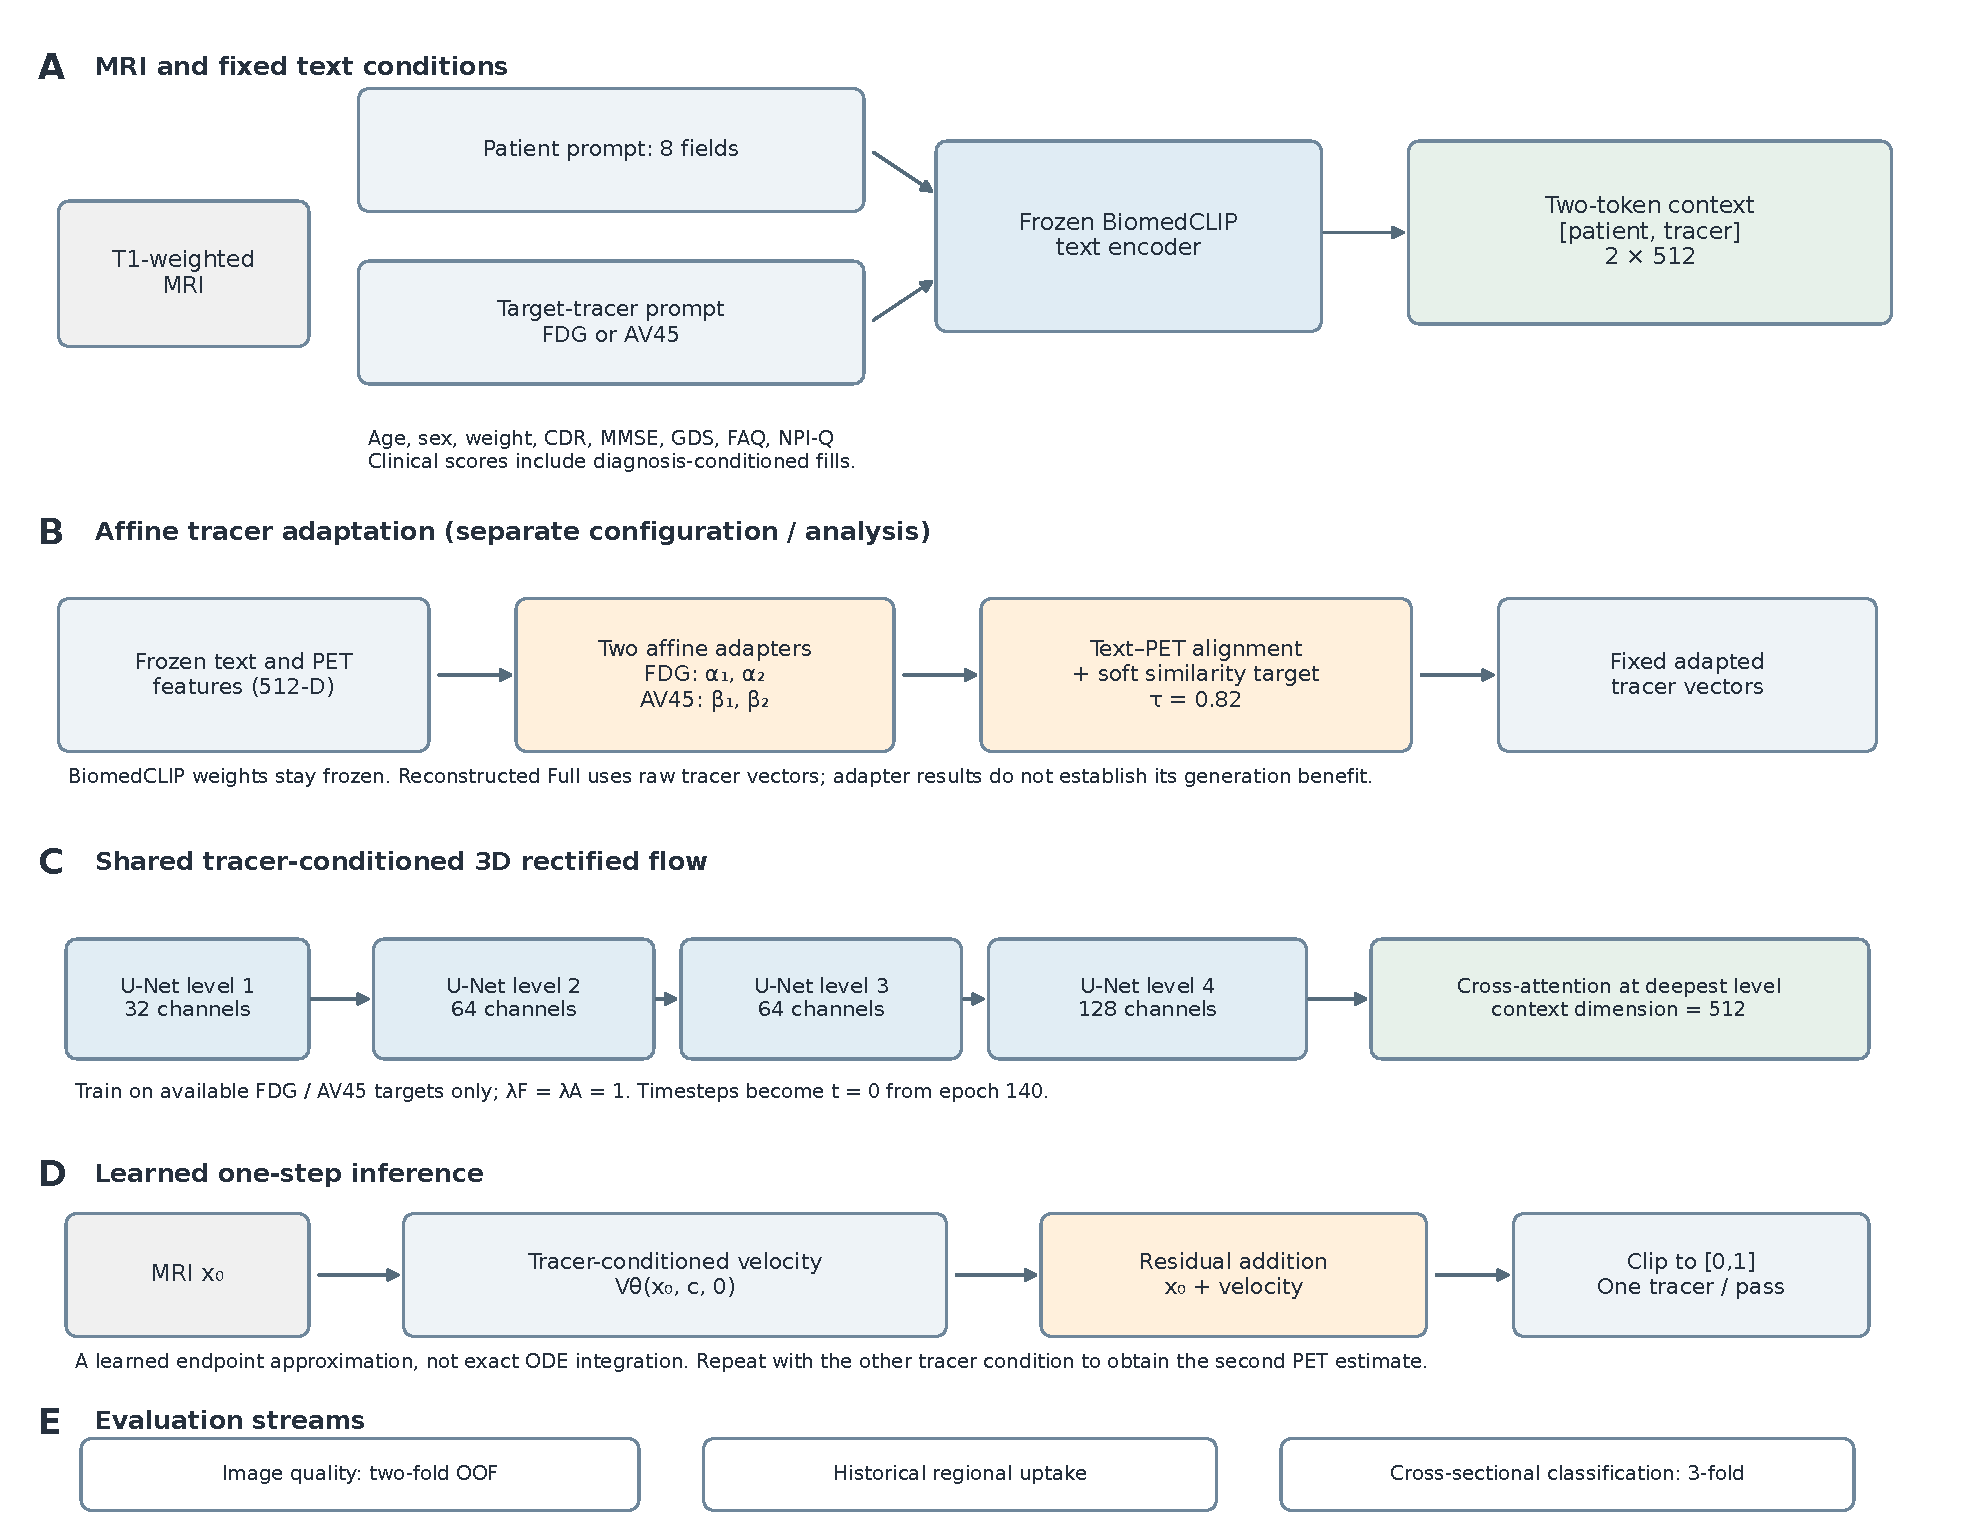
\includegraphics[width=\textwidth]{figure_1}
    \caption{\textbf{Overview of the DIReCT$++$ framework for multimodal PET synthesis and downstream analysis.}
(A) Tracer-conditioned rectified flow from MRI to FDG- or AV45-PET. (B) Lightweight affine fine-tuning of tracer guidance derived from frozen BiomedCLIP encoders. The symbols $\alpha$ and $\beta$ denote FDG adapter parameters $(\alpha_1,\alpha_2)$ and AV45 adapter parameters $(\beta_1,\beta_2)$, respectively; these adaptations are separate from the raw tracer embeddings used by the reconstructed Full generation experiments. (C) A shared conditional 3D U-Net predicts velocity fields for the requested tracer. (D) Learned one-step PET estimation by residual addition of the predicted velocity to MRI; each forward pass produces one tracer. (E) Image-quality, regional uptake and cross-sectional classification analyses. These analyses do not establish clinical replacement of PET.}
    \label{fig:1}
\end{figure}

\subsection{PET Synthesis Quality and External Evaluation}
PET synthesis was evaluated using structural similarity (SSIM), peak signal-to-noise ratio (PSNR), mean squared error (MSE) and mean absolute error (MAE). Figure~\ref{fig:2} retains the historical comparisons with CycleGAN~\cite{zhu2017unpaired}, Swin-UNet~\cite{Cao2021swin}, segmentation-guided diffusion~\cite{konz2024anatomically}, 3D DDIM~\cite{song2021ddim,pinaya2023generative}, 3D rectified flow~\cite{Xing2022} and single-tracer DIReCT~\cite{liu2025direct}. Absolute historical aggregate values are given in Table~\ref{tab:historical_generation}; subject-level statistics were not recoverable for every historical method and are not reconstructed from these aggregates.
PET synthesis used two-fold ADNI evaluation; historical external evaluation used OASIS-3 AV45 only. The reconstructed OOF comparisons and their statistical protocols are reported separately from the historical Figure~\ref{fig:2} summaries.

The reconstructed OOF evaluation does not support a uniform advantage of Full over all alternatives (Tables~\ref{tab:whole_volume_generation},\ref{tab:paired_generation}). Full outperformed the clinically conditioned regression U-Net across the four whole-volume metrics for both tracers, while the magnitude of the AV45 MSE effect was small ($|d_z|=0.075$). Relative to TabularMLP, Full had higher SSIM but lower PSNR and higher MSE for both tracers; MAE did not differ after the specified Holm correction. TracerOnly had better FDG results on all four metrics and higher AV45 SSIM than Full. Single-tracer DIReCT had higher FDG SSIM, whereas Full had better FDG PSNR/MSE and AV45 SSIM. These independently trained models differ in initialization, conditioning or implementation, so the comparisons do not isolate a single causal component or prove multi-tracer synergy.

In the masked evaluation (Tables~\ref{tab:r3_11_masked_summary},\ref{tab:r3_11_masked_paired}), Full had higher mean SSIM/PSNR and lower mean MSE/MAE than Clinical U-Net and MRI-only Swin-UNETR for both tracers; all 16 predefined comparisons met $p_{\mathrm{Holm}}<0.05$ within their two separate eight-test families. The masked cohort contained 1,597 FDG and 1,364 AV45 observations after the existing MRI/mask QC exclusion. For Clinical U-Net AV45 MSE/MAE, the standardized effects were small ($|d_z|=0.071/0.076$), and only 56.4--57.8\% of subjects favored Full. Thus statistical support does not imply uniform individual or clinical benefit. Full/Clinical U-Net used epoch 165, while MRI-only Swin-UNETR used epoch 200; information and training endpoints differ.

Separate whole-volume and masked summaries are retained because background exclusion changes the metric definitions and values. Supplemental FDG and AV45 examples use the median, 10th-percentile and worst QC-passed subjects selected by saved whole-volume SSIM, and show MRI, real PET, synthetic PET and absolute-error maps (Figs.~\ref{fig:cases_fdg},\ref{fig:cases_av45}).

The historical OASIS-3 evaluation reports AV45 PSNR of 26.79 dB, compared with 28.09 dB for historical internal ADNI AV45 evaluation (Fig.~\ref{fig:2}A; Table~\ref{tab:historical_generation}). The cross-dataset examples in Fig.~\ref{fig:2}C illustrate CN/AD AV45 synthesis. These aggregate and illustrative results do not provide subject-level confidence intervals, FDG external evidence or external MCI-stage validation, and should not be combined with the reconstructed OOF statistics as a single experiment.

\begin{figure}[htbp]
\centering
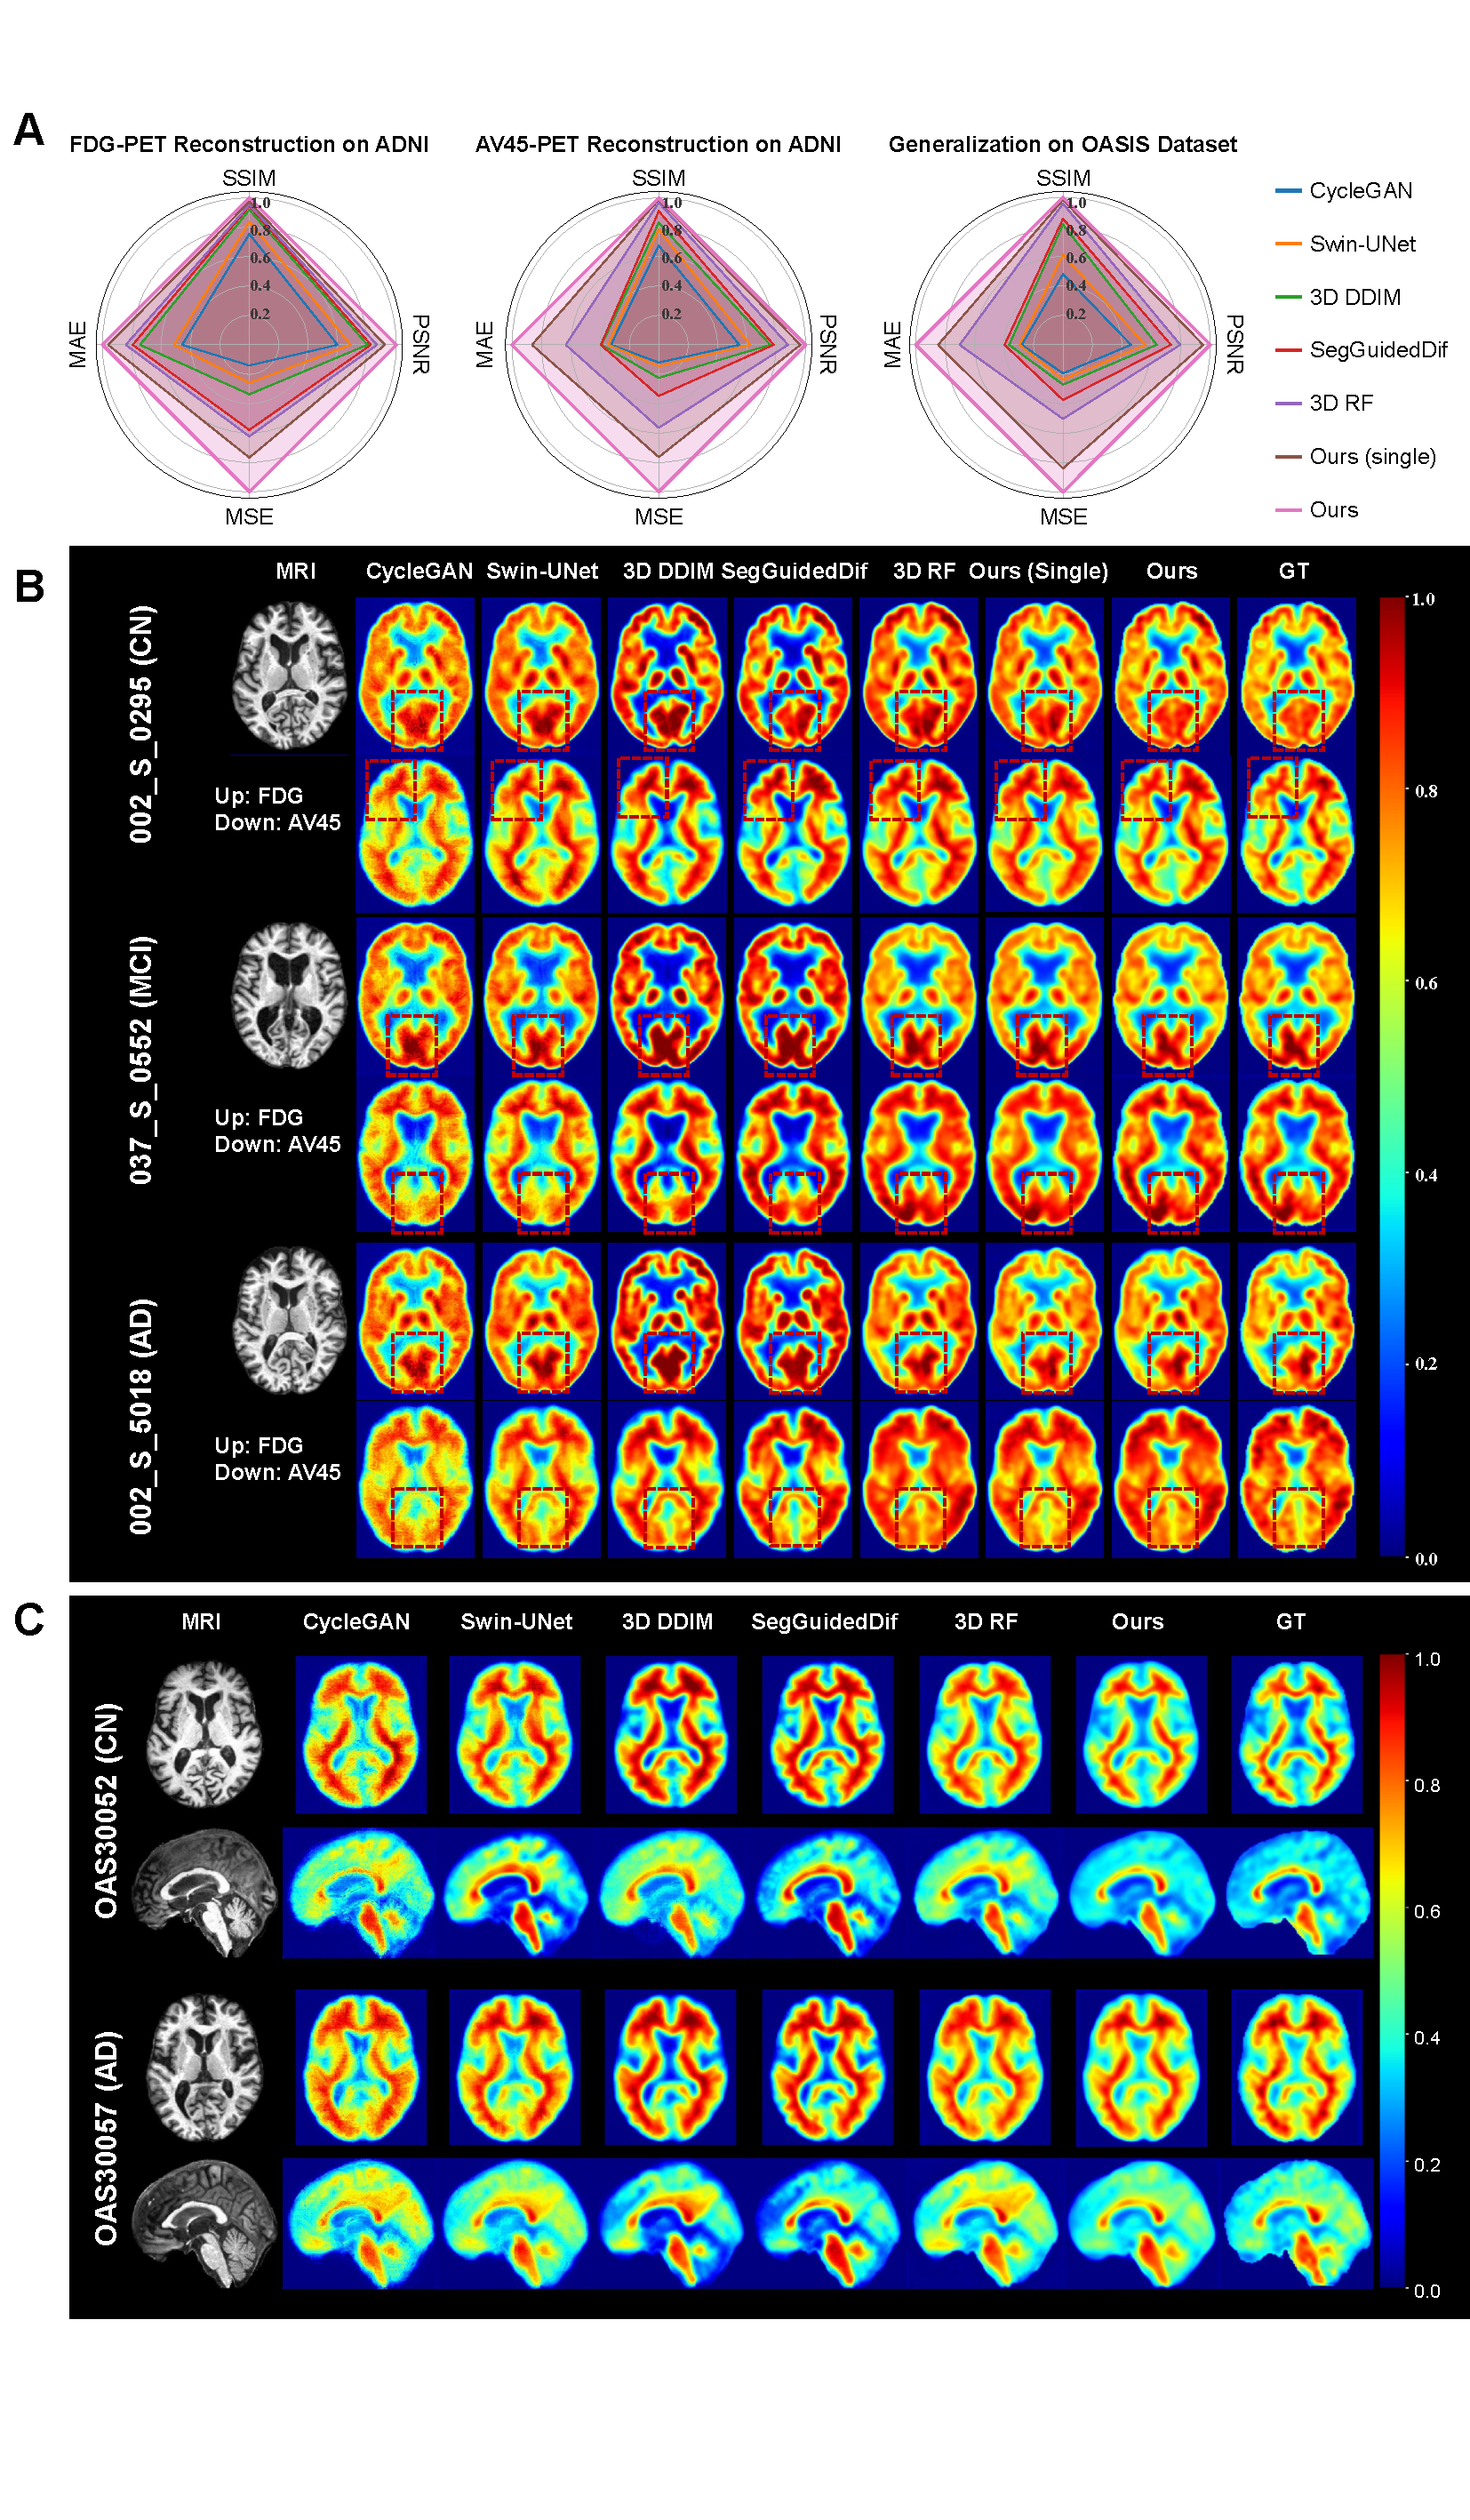
\includegraphics[width=\textwidth,height=.62\textheight,keepaspectratio]{figure_2}
\caption{\textbf{Historical PET synthesis comparisons and illustrative examples.} (A) Radar plots summarize the historical aggregate SSIM, MSE, MAE and PSNR values for ADNI FDG/AV45 and OASIS-3 AV45. Metric values are displayed relative to the best value among methods; absolute aggregate values and scaling conventions are listed in Table~\ref{tab:historical_generation}. These aggregates are separate from the reconstructed OOF and masked analyses. (B) Illustrative ADNI CN, MCI and AD examples with MRI, competing synthesis outputs and real PET; paired subrows show FDG and AV45. (C) Historical CN/AD OASIS-3 examples are limited to AV45. Examples were randomly selected within diagnostic groups as reported by the authors; the selection seed could not be verified from the available records. This differs from the supplemental quantile-based selection and does not establish population-level superiority.}
\label{fig:2}
\end{figure}

% Source-backed publication fragment; source records retained independently.
% Source: reports/baseline_metrics_provenance_20261020/paper_figure2_values.csv
\begingroup
\footnotesize
\setlength{\tabcolsep}{4pt}
\begin{longtable}{llllll}
\caption{Absolute historical Figure 2 summary values}\label{tab:historical_generation}\\
\toprule
cohort & method & SSIM\_percent & PSNR & MSE\_percent & MAE\_percent \\
\midrule
\endfirsthead
\toprule
cohort & method & SSIM\_percent & PSNR & MSE\_percent & MAE\_percent \\
\midrule
\endhead
\bottomrule
\endfoot
ADNI\_FDG & Cyclegan & 67.82 & 17.26 & 2.35 & 6.47 \\
ADNI\_FDG & Swin-Unet & 75.29 & 19.82 & 1.27 & 5.76 \\
ADNI\_FDG & DDIM(3D) & 82.62 & 23.09 & 0.98 & 3.98 \\
ADNI\_FDG & SegGuidedDif & 84.85 & 23.76 & 0.57 & 3.73 \\
ADNI\_FDG & Rectified Flow & 85.69 & 24.96 & 0.53 & 3.52 \\
ADNI\_FDG & Ours(single) & 87.48 & 26.51 & 0.43 & 3.08 \\
ADNI\_FDG & Ours & 89.94 & 28.72 & 0.33 & 2.96 \\
ADNI\_AV45 & Cyclegan & 59.56 & 15.43 & 3.24 & 8.39 \\
ADNI\_AV45 & Swin-Unet & 69.16 & 17.54 & 2.67 & 7.95 \\
ADNI\_AV45 & DDIM(3D) & 73.37 & 21.33 & 1.73 & 7.01 \\
ADNI\_AV45 & SegGuidedDif & 80.29 & 21.99 & 1.12 & 6.92 \\
ADNI\_AV45 & Rectified Flow & 85.43 & 24.74 & 0.69 & 4.31 \\
ADNI\_AV45 & Ours(single) & 87.37 & 27.11 & 0.51 & 3.16 \\
ADNI\_AV45 & Ours & 88.21 & 28.09 & 0.39 & 2.73 \\
OASIS & Cyclegan & 40.27 & 12.38 & 4.86 & 10.78 \\
OASIS & Swin-Unet & 51.34 & 14.96 & 3.96 & 10.16 \\
OASIS & DDIM(3D) & 68.59 & 17.05 & 3.48 & 8.24 \\
OASIS & SegGuidedDif & 71.85 & 19.63 & 2.51 & 7.59 \\
OASIS & Rectified Flow & 80.44 & 21.33 & 1.87 & 4.29 \\
OASIS & Ours(single) & 82.66 & 25.48 & 1.12 & 3.55 \\
OASIS & Ours & 83.97 & 26.79 & 0.94 & 3.01 \\
\end{longtable}
\noindent\parbox{\linewidth}{\footnotesize 21method/cohort rows x4metrics =84historical values. SSIM/MSE/MAE retain source percent scales, PSNR dB. OASIS is AV45 only. No recovered common per-subject final inputs: SD, CI and paired p unavailable. These are not the fixed W1 OOF experiment and are not paired with it. Original radar figure unchanged.}
\endgroup


\subsection{Recapitulation of Disease-Specific Biomarker Patterns}
To assess regional uptake patterns, the corresponding T1-weighted MRI scans were parcellated using SynthSeg~\cite{synthseg}, and the resulting Desikan--Killiany and \textit{aseg} ROI masks were applied to spatially aligned real and synthetic PET images. This approach yielded a total of 98 distinct regions of interest (ROIs), including cortical, subcortical, cerebellar, and brainstem structures. Regional normalized uptake values (arbitrary units) were computed as the mean voxel intensity within each ROI from PET images normalized using per-image min--max intensity scaling. Fig.~\ref{fig:3} illustrates this analysis for key ROIs in two representative ADNI subjects, illustrating regional patterns in these selected cases.

\begin{figure}[htbp]
    \centering
    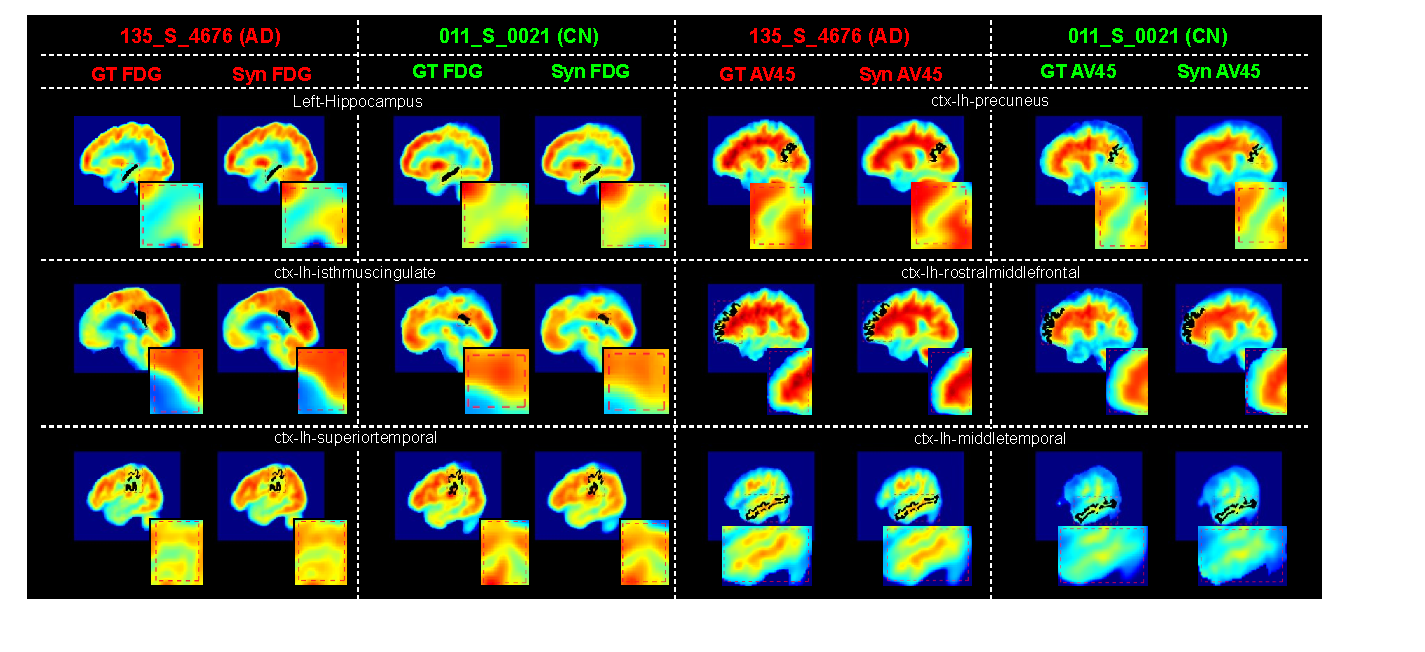
\includegraphics[width=\textwidth]{figure_3}
    \caption{
\textbf{Detailed regional visualization of synthetic and real PET images.}
The figure displays magnified regional views of FDG-PET (left two columns) and AV45-PET (right two columns) for representative AD and CN subjects. 
For each modality and group, the first sub-column shows real PET, and the second sub-column shows synthetic PET. 
Key anatomical regions are highlighted in the bottom-right corner of each sub-column, with their names labeled at the top-center. 
Each row corresponds to a distinct brain region. Displayed uptake values are arbitrary units after per-image min--max normalization, without anatomical reference-region normalization. Cases were randomly selected within their diagnostic groups as reported by the authors; the selection seed could not be verified from the available records. These selected cases illustrate regional appearance and do not establish population-level agreement or clinical SUV/SUVR calibration.
}
    \label{fig:3}
\end{figure}

For a comprehensive quantitative evaluation, we performed two complementary regional statistical analyses on the ADNI cohort. First, we compared synthetic and real images to assess the normalized regional uptake agreement of DIReCT$++$. Second, we compared the AD and CN groups separately in real and synthetic PET to assess whether disease-related regional differences were retained. Figure~\ref{fig:4}A,B uses the pooled available subjects without diagnostic-group stratification; panels C--F compare AD and CN only.

Paired-sample $t$-tests between synthetic and real images revealed no statistically significant differences in normalized regional uptake across the principal brain regions shown in Fig.~\ref{fig:4}A, B for the overall cohorts of both tracers ($p>0.05$). Across all 98 ROIs, no overall comparisons remained significant after Benjamini--Hochberg false discovery rate (FDR) correction (all $q>0.05$). Among the diagnosis-stratified paired comparisons, only the right pericalcarine cortex (ROI 2021) in the $^{18}$F-FDG MCI subgroup showed a significant mean paired difference after FDR correction ($q=0.0481$). The median concordance correlation coefficients (CCC) across the 98 ROIs were 0.9745 for $^{18}$F-AV-45 and 0.9450 for $^{18}$F-FDG, with corresponding median mean absolute errors (MAE) of 0.0160 and 0.0159 (normalized intensity units). For the 16 representative tracer--ROI combinations in Fig.~\ref{fig:4}A, B, descriptive regression slopes ranged from 0.9794 to 1.0127 (median, 1.0007) for $^{18}$F-AV-45 and from 0.9844 to 1.0101 (median, 1.0001) for $^{18}$F-FDG, without a consistent direction of deviation from unity. These results indicate close agreement in normalized regional uptake between synthetic and real PET, with detailed statistics for the representative ROIs provided in Supplementary Table~\ref{tab:regional_agreement}. Non-significant mean differences do not establish formal equivalence or clinical interchangeability. These historical regional-CSV results are separate from the reconstructed Full generation comparisons.

Critically, independent-sample $t$-tests demonstrated that the significant differences between diagnostic groups observed in real PET data were also observed in the synthetic images (Fig.~\ref{fig:4}C, D; figs.~\ref{fig:supp_disease_av45} and \ref{fig:supp_disease_fdg}). For instance, DIReCT$++$ recapitulated the statistically significant differences between AD and CN groups in the left precuneus for $^{18}$F-AV-45 (real: $q=7.73\times10^{-66}$; synthetic: $q=1.25\times10^{-63}$; Fig.~\ref{fig:4}C) and in the left hippocampus for $^{18}$F-FDG (real: $q=4.27\times10^{-15}$; synthetic: $q=1.27\times10^{-13}$; Fig.~\ref{fig:4}D). Similarly, regional differences that were non-significant in real PET data remained non-significant in the synthetic images after FDR correction (all $q\geq0.05$ for the regions shown in Fig.~\ref{fig:4}E, F). The AD--CN effect-size directions were consistent between real and synthetic PET for all ten regions shown in Fig.~\ref{fig:4}C, D, although the absolute Cohen's $d$ decreased in nine regions (maximum reduction, 0.0771). These findings support the preservation of group-level disease-related regional uptake patterns, while indicating variations in effect-size magnitude. Complete effect-size estimates and FDR-adjusted results for the displayed regions are provided in Supplementary Table~\ref{tab:regional_effect_sizes}. The AD--CN comparison illustrates representative differences between two diagnostic states rather than all diagnostic-group contrasts. MCI was evaluated separately through MCI-versus-CN and EMCI-versus-LMCI classification (Fig.~\ref{fig:5}B,C); the regional paired analysis also includes the original MCI categories.

\begin{figure}[htbp]
\centering
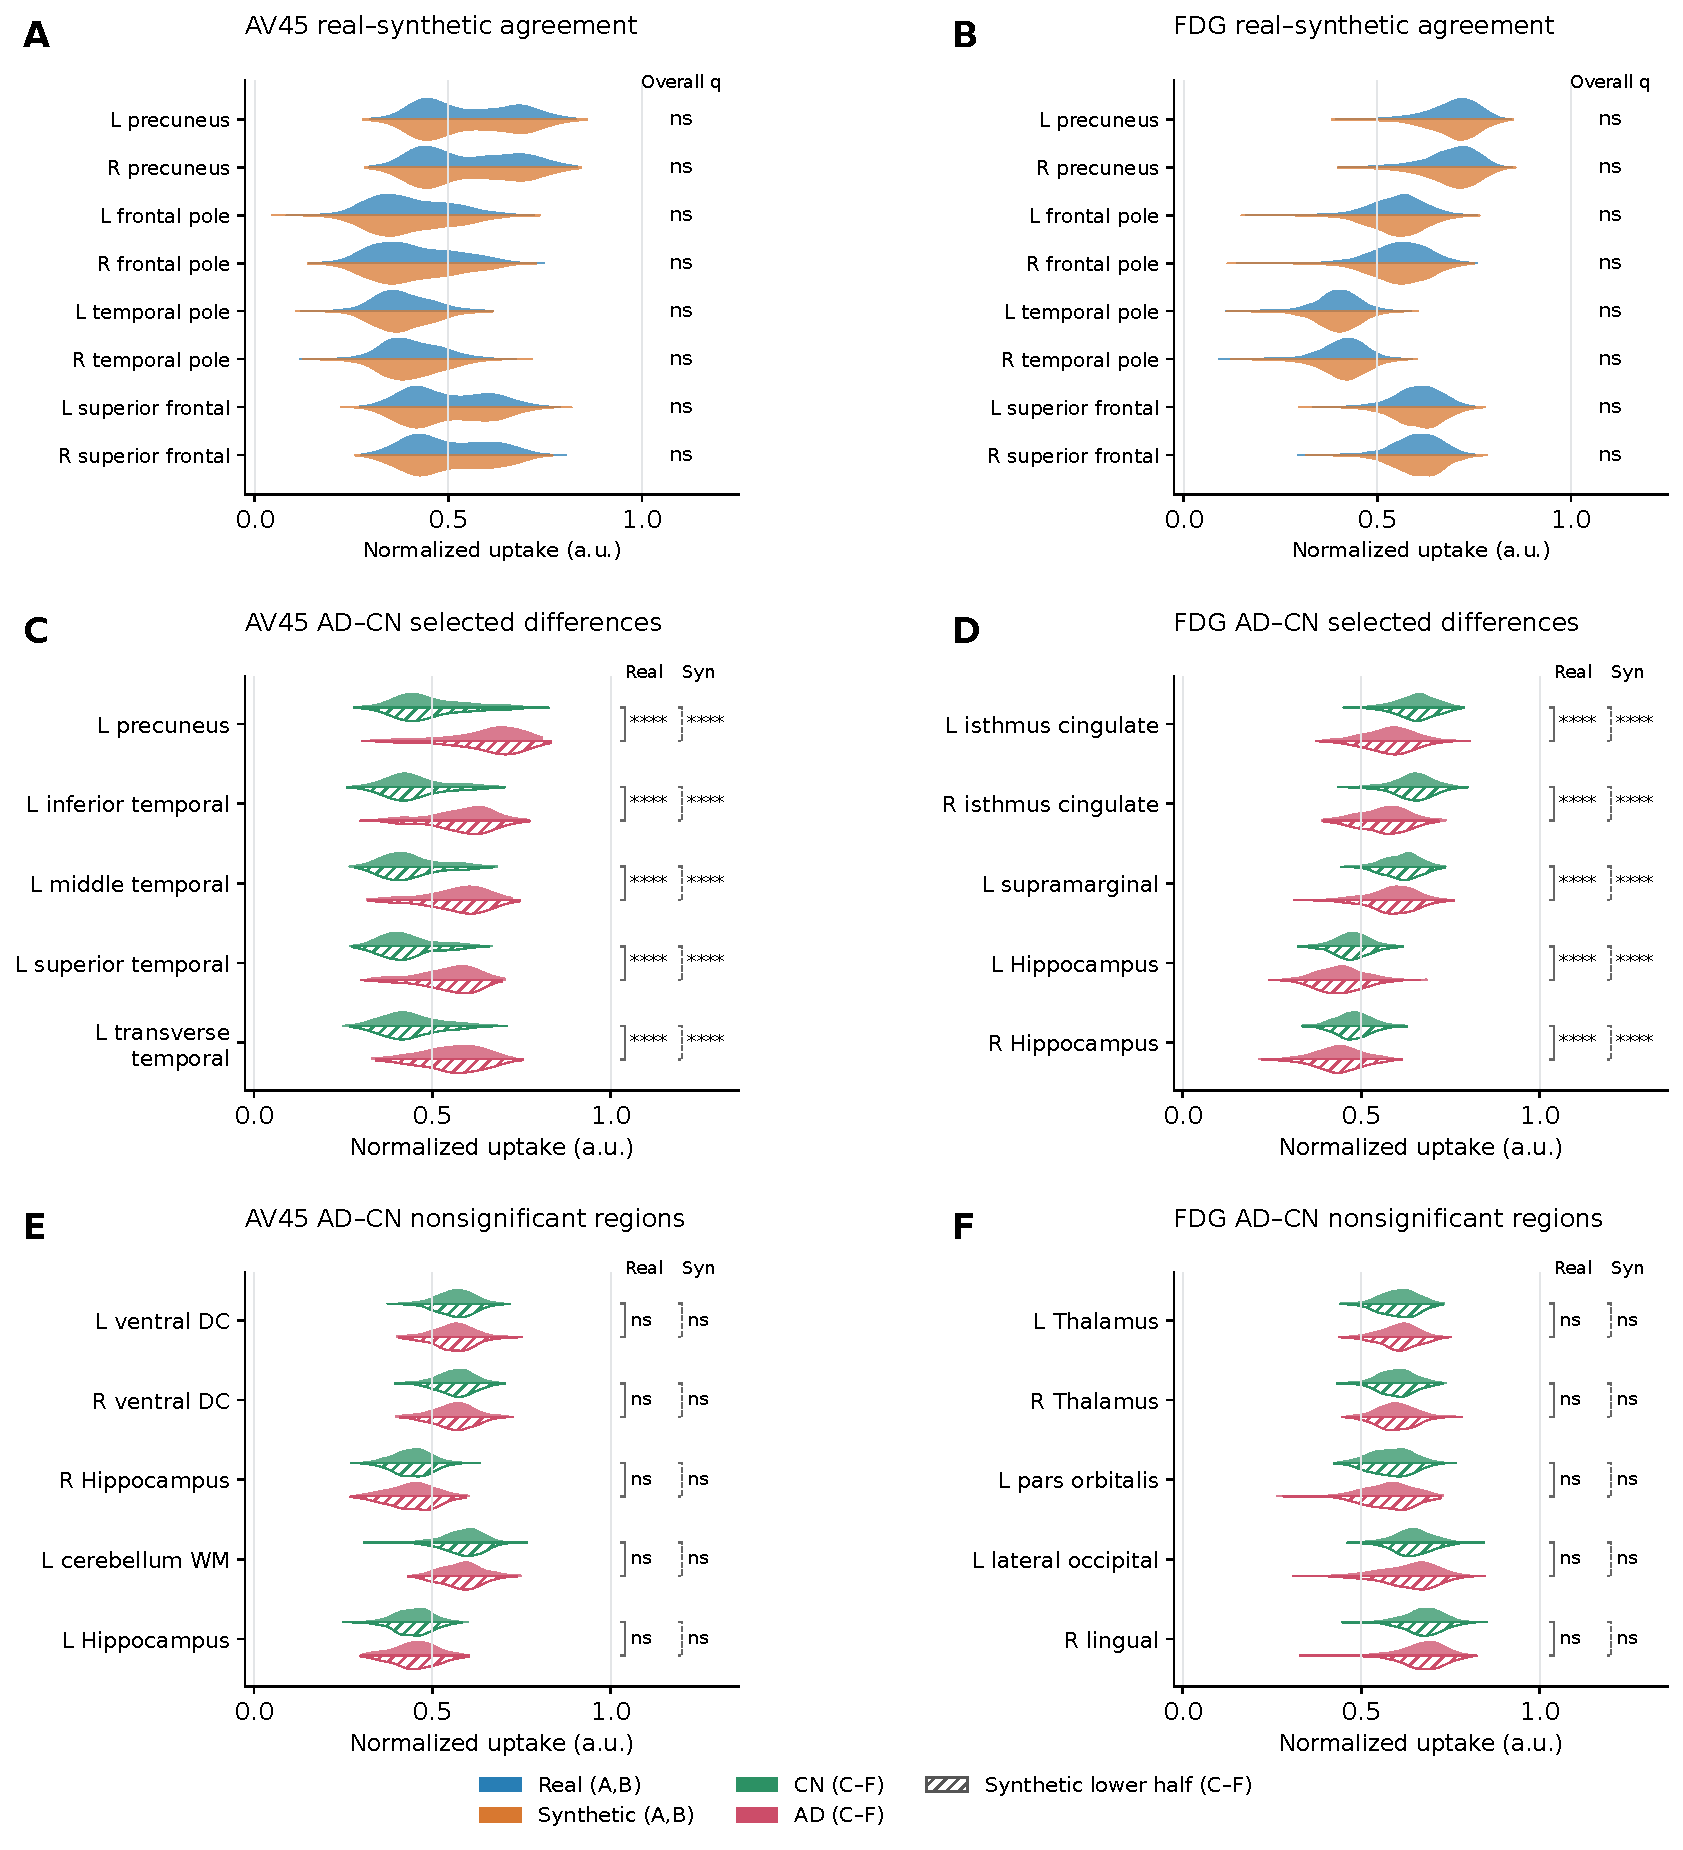
\includegraphics[width=\textwidth,height=.62\textheight,keepaspectratio]{figure_4}
\caption{
\textbf{Regional comparison of mean normalized uptake between real and MRI-synthetic PET images.}
(A,B) Violin plots show regional mean normalized uptake (arbitrary units) across cortical and subcortical regions for real and synthetic PET, comparing AV45 (A) and FDG (B). All regional uptake values were derived from per-image min--max-normalized PET intensities without anatomical reference-region normalization.
Panels A,B summarize the pooled available subjects without diagnostic stratification. Non-significant differences are not evidence of equivalence. (C--F) AD--CN regional comparisons. Violin plots display mean normalized uptake in AD (red) and CN (green) subjects for selected regions. Each region uses paired half-violins: upper (solid) = real PET, lower (hatched) = synthetic PET; colors match across modalities. Solid lines indicate real PET significance, dashed lines indicate synthetic PET significance. The statistical annotations in panels (C--F) follow the BH-FDR analysis: \texttt{****} corresponds to $q<10^{-4}$ and \texttt{ns} to $q\geq0.05$. (C,D) show representative regions with significant AD--CN differences for AV45 and FDG, whereas (E,F) show selected regions without significant AD--CN differences after FDR correction. Cblm-WM denotes Cerebellum-White-Matter. The figure was recreated from the author-designated regional CSVs using the reported BH-FDR reanalysis; it is not claimed to recover the exact historical drawing files. Additional regional agreement and effect-size analyses are provided in the Supplementary Materials.
}
\label{fig:4}
\end{figure}

\subsection{Diagnostic Classification and MCI Stage Discrimination}
Classification used independent subject-level three-fold evaluation for AD versus CN ($n=470$), EMCI+LMCI versus CN ($n=741$), and EMCI versus LMCI ($n=436$). The MCI/CN task includes EMCI and LMCI, while MCI-U is excluded. The completed analysis comprises 63 imaging and 18 clinical fits (27 task--input configurations, three folds each). Results are reported as the equally weighted fold mean $\pm$ sample s.d., alongside conditional bootstrap 95\% CIs (Table~\ref{tab:classification_summary}). This is cross-sectional MCI stage discrimination, not future conversion or longitudinal prognostic prediction.

For AD/CN, MRI+Syn-FDG+Syn-AV45 achieved ACC $88.08\pm2.06\%$ and AUC $93.82\pm3.21\%$, compared with MRI-only ACC $79.56\pm6.20\%$ and AUC $87.02\pm5.44\%$ (Fig.~\ref{fig:5}A). The paired AUC difference was $+6.80$ percentage points (95\% CI $[+3.39,+10.22]$). For MCI/CN, MRI+Syn-both had ACC $65.45\pm1.64\%$ and AUC $69.46\pm1.34\%$, versus MRI-only $67.48\pm0.23\%$ and $71.59\pm1.80\%$; the paired AUC difference was $-2.13$ points (95\% CI $[-6.30,+2.10]$; Fig.~\ref{fig:5}B). Thus the synthetic combination did not improve all tasks.

For EMCI/LMCI, MRI+Syn-both had ACC $65.82\pm2.06\%$ and AUC $66.33\pm0.54\%$, compared with MRI-only $64.90\pm3.09\%$ and $62.81\pm2.50\%$. Its balanced-ACC difference favored the synthetic combination by $6.91$ points (95\% CI $[2.02,11.98]$), while the ACC and AUC difference CIs crossed zero (Fig.~\ref{fig:5}C). The Syn-minus-Real dual-PET AUC intervals crossed zero for all three tasks, which does not establish equivalence or interchangeability (Table~\ref{tab:classification_comparisons}).

Clinical-only AUC was $100.00\pm0.00\%$ for AD/CN, $98.93\pm0.70\%$ for MCI/CN, and $99.94\pm0.08\%$ for EMCI/LMCI. MRI+Clinical AUC was $99.17\pm0.96\%$, $93.07\pm6.10\%$, and $89.60\pm9.08\%$, respectively. MRI+Syn-both AUC was below both clinical baselines in each task, with the specified paired intervals below zero. These observations do not support independent incremental diagnostic value over the clinical variables, which include diagnosis-related scores and diagnosis-conditioned fills. The zero observed AD/CN error for Clinical-only and its degenerate empirical bootstrap CI do not establish perfect population generalization.

\begin{figure}[htbp]
\centering
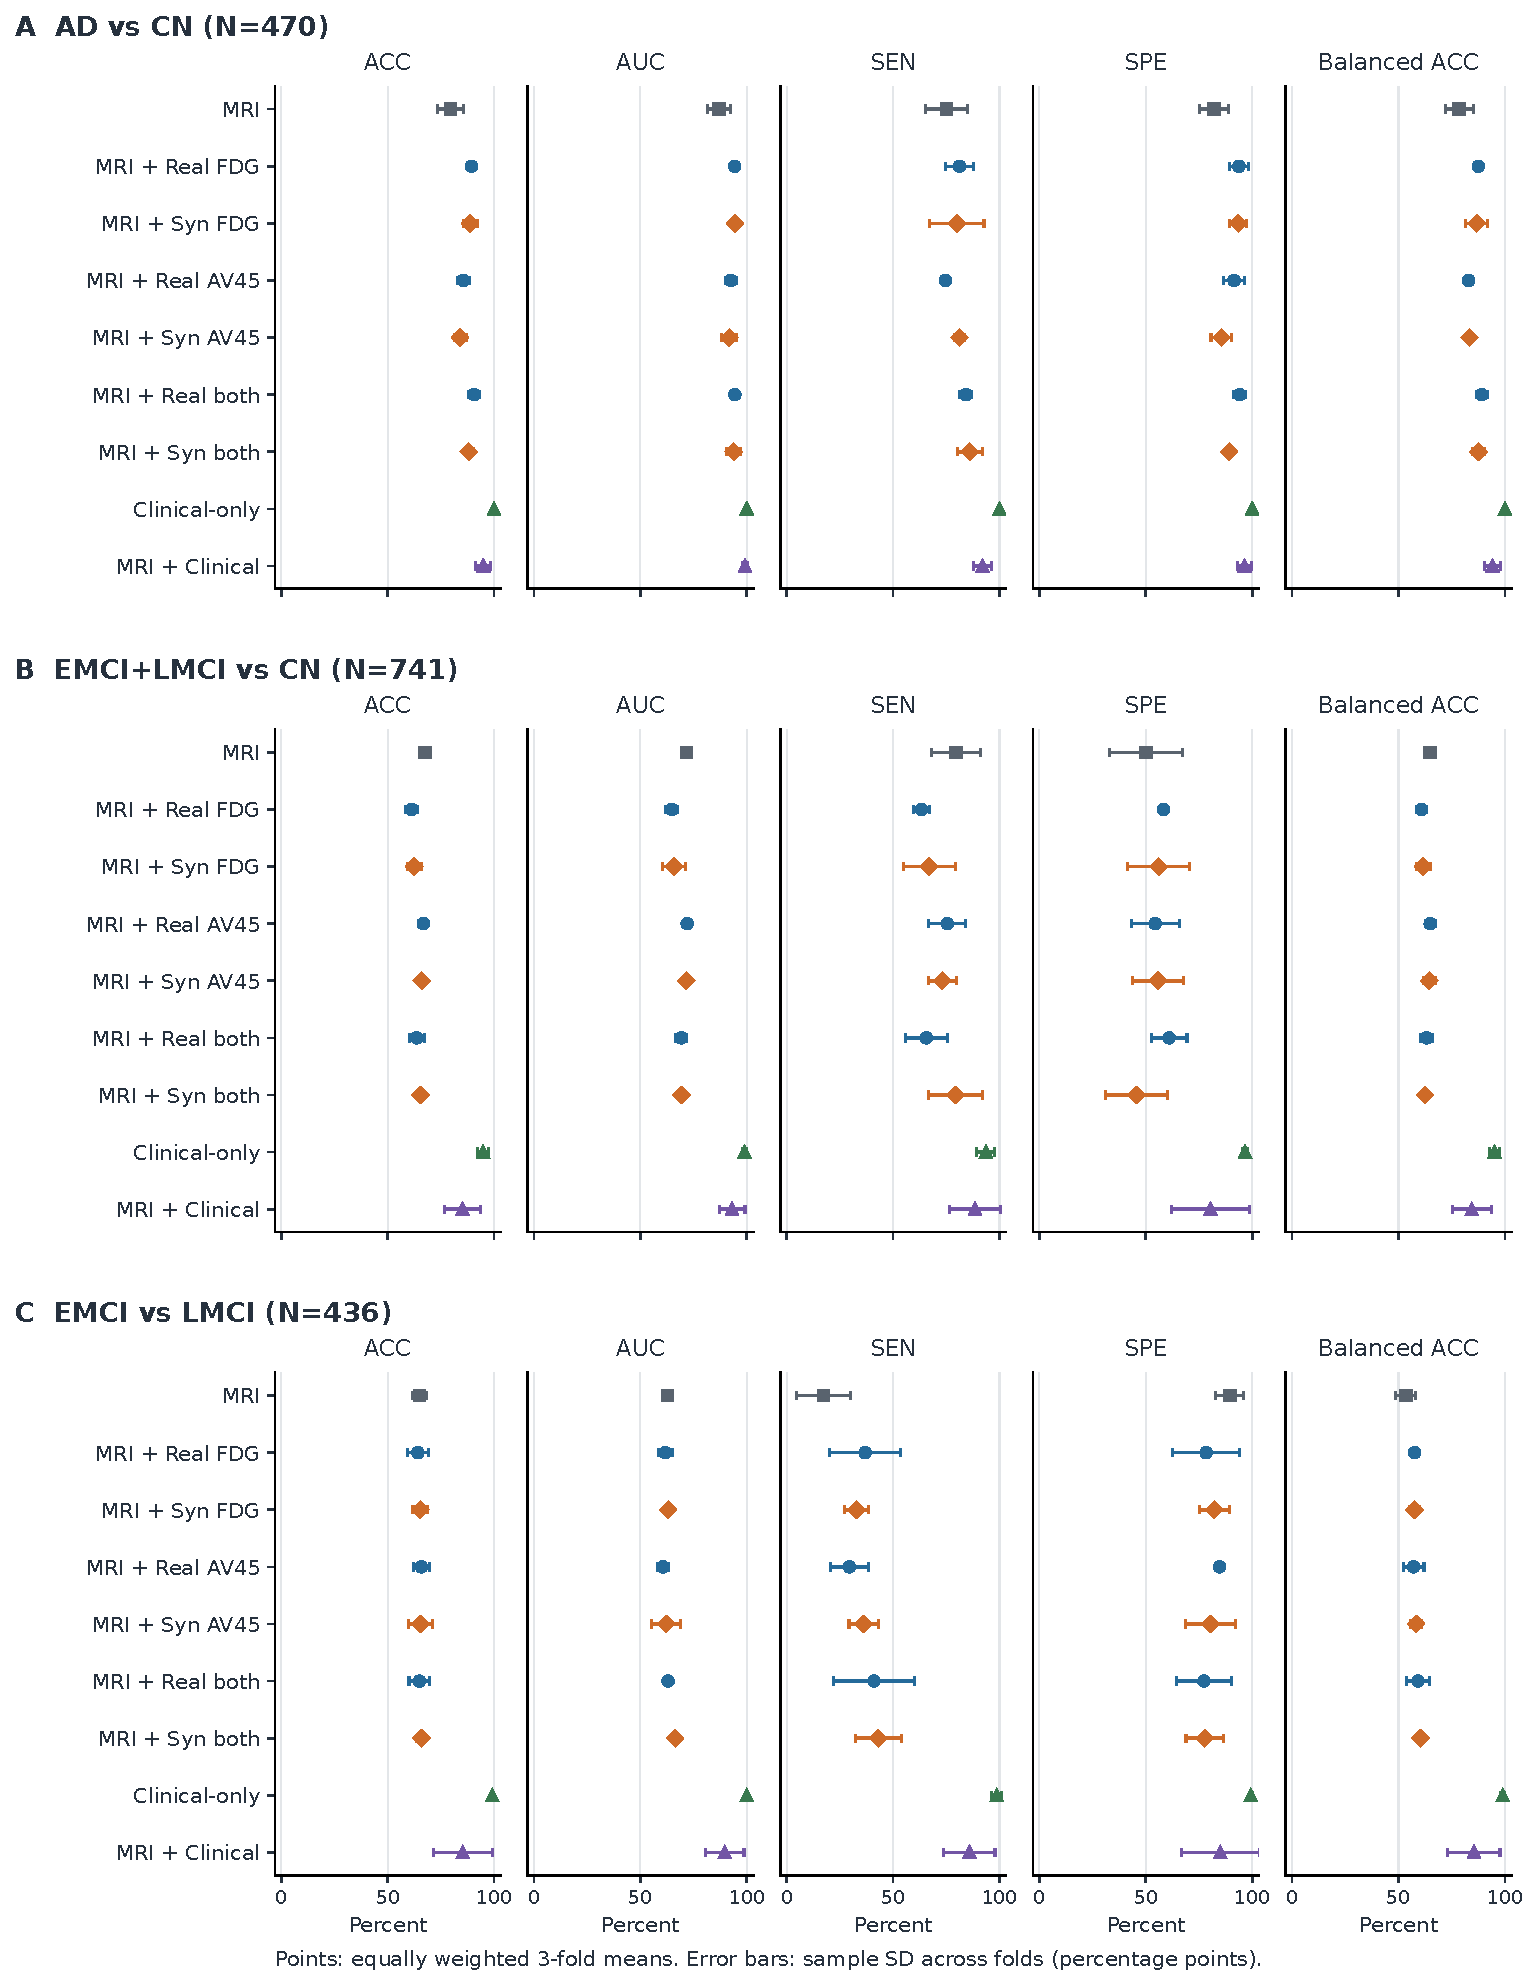
\includegraphics[width=\textwidth,height=0.68\textheight,keepaspectratio]{figure_5}
\caption{\textbf{Cross-sectional classification under the revised three-fold protocol.} Rows A--C correspond to AD/CN, EMCI+LMCI/CN and EMCI/LMCI. Within each row, the five metric columns compare nine input conditions: MRI; MRI+Real FDG; MRI+Syn FDG; MRI+Real AV45; MRI+Syn AV45; MRI+Real-both; MRI+Syn-both; Clinical-only; and MRI+Clinical. Points are equally weighted three-fold means; horizontal error bars show sample s.d. in percentage points, not 95\% CIs. ACC, AUC, SEN, SPE and balanced ACC are reported with their CIs in Table~\ref{tab:classification_summary}. The results do not demonstrate longitudinal prognosis, PET equivalence or benefit independent of diagnosis-related clinical inputs.}
\label{fig:5}
\end{figure}

Supplemental ROC curves use fold-wise averaging and pointwise confidence bands (Fig.~\ref{fig:classification_roc}). Paired DeLong tests are reported by outer fold with their raw and family-specific Holm-adjusted $p$ values (Table~\ref{tab:classification_delong}); they are not combined into a three-fold overall DeLong test. All comparisons are conditional on the fixed trained models and splits.

Age ($<75$ versus $\geq75$ years) and sex were analyzed separately using existing classification predictions (Tables~\ref{tab:r2-16-ad-cn},\ref{tab:r2-16-mci-cn},\ref{tab:r2-16-emci-lmci}). For AD/CN, MRI+Syn-both minus MRI balanced-ACC differences ranged from 7.45 to 10.97 percentage points across the four subgroups. EMCI/LMCI point differences were positive in all four subgroups, including 9.64 points for age $\geq75$ (95\% CI $[1.23,18.05]$); MCI/CN did not show consistent gains. The subgroup intervals are marginal and unadjusted. These stratified descriptions do not remove demographic confounding or establish age/sex interactions.



\section{Discussion}
DIReCT$++$ combines shared tracer-conditioned 3D rectified flow with biomedical text guidance for FDG- and AV45-PET synthesis from MRI. Its contribution extends the single-tracer DIReCT framework to multi-tracer modeling and a separately evaluated affine-adapter formulation. The evidence comprises historical aggregate comparisons, reconstructed OOF generation, normalized regional uptake statistics and a separate cross-sectional classification analysis. These sources should be interpreted within their respective input and execution identities rather than as a single verified historical run.

The generation results show both advantages and tradeoffs. Full had better masked image-quality means than the clinical regression U-Net and MRI-only Swin-UNETR, while some AV45 error effects were small and did not imply universal individual benefit. Whole-volume comparisons favored TabularMLP for PSNR/MSE and TracerOnly for several endpoints. The adapter analysis supports control of tracer-embedding geometry, but it does not establish a causal improvement in PET generation. Fixed-weight conditioning interventions indicate that patient features can influence outputs; independently initialized Full/TracerOnly or text/tabular models do not isolate the clinical or VLM component as the sole cause of their performance differences.

The potential value of this framework is to improve access to biomarker-related imaging information for multimodal imaging research. The classification findings are task dependent: MRI+Syn-both improved AD/CN relative to MRI, did not improve MCI/CN, and showed mixed EMCI/LMCI endpoints. Clinical-only and MRI+Clinical AUC exceeded MRI+Syn-both in the completed comparisons. Because clinical inputs include diagnosis-related assessments and diagnosis-conditioned fills, these findings cannot be used to establish independent diagnostic value of synthetic PET. Similar observed Real/Syn performance does not demonstrate equivalence or molecular validity.

Synthetic PET may support exploratory MRI-based analyses when PET is unavailable, but clinical screening or treatment selection would require independent molecular biomarker confirmation and prospective validation. No longitudinal conversion, progressive-versus-stable MCI, survival or treatment-response endpoints were analyzed. EMCI/LMCI classification is therefore MCI stage discrimination; it does not predict an individual's progression to AD. Whether serially synthesized PET can reflect progression or treatment response remains a question for longitudinal studies.

Within medical image synthesis, DIReCT$++$ evaluates disease-related regional uptake patterns and downstream classification in addition to image-level metrics. The shared flow model and biomedical conditioning provide a framework for further study, rather than establishing clinically actionable biomarkers or attributing all overall differences to one architectural component. The learned one-step approximation permits a single tracer-conditioned forward pass; measured forward latency does not constitute an end-to-end workflow or an equal-protocol speedup over competing models.

Several limitations require explicit consideration. Clinical-record reconstruction showed extensive diagnosis-conditioned filling of missing scores, which can introduce group information into conditioning and classification. Source weight entries also contain unresolved validity issues. The original random filling states and complete actual acquisition mappings were not recovered. The independent three-fold classifier evaluation verifies its own partitions, but the historical synthetic-image inputs could not be bound directly to the checkpoints in the reconstructed generation comparisons. These limitations constrain claims of reproducibility and independent clinical discrimination.

Regional measurements use per-image min--max-normalized intensities in arbitrary units, without established anatomical-reference SUV/SUVR calibration. No clinically justified equivalence margin, formal TOST result or valid amyloid-positivity agreement analysis was established. Close agreement, non-significant paired differences or preservation of AD--CN significance is not evidence of clinical equivalence or reliable atypical A$\beta$ status classification. Calibrated quantitative PET and prespecified, clinically meaningful equivalence margins are needed for such assessments.

The deterministic one-step formulation provides a single output per input without calibrated subject-level predictive uncertainty. An MSE-trained deterministic model may represent an average conditional mapping and cannot guarantee recovery of individual molecular pathology from MRI and text. Ensemble or stochastic uncertainty estimation remains future work. Not all requested single-component ablations or matched one-step/multistep evaluations were completed. The fixed-model bootstrap intervals do not quantify training-seed or split variability.

External evaluation was limited to historical AV45 synthesis in OASIS-3 CN/AD, with age differences and incomplete run-specific prompt records; FDG and MCI external generalizability remain unestablished. Prospective validation in more diverse clinical populations, including alternative MRI acquisitions~\cite{sorby2024portable}, is needed. Additional clinical modalities such as blood biomarkers~\cite{hansson2023blood} may provide complementary information, but their incremental value must be evaluated independently. The 2024 Alzheimer's Association criteria emphasize biological diagnosis using validated core biomarkers, including amyloid PET and sufficiently accurate blood-based assays such as plasma p-tau217~\cite{jack2024revised}. Synthetic PET has not been validated as a substitute for molecular confirmation, and its added value relative to those biomarker assessments remains to be determined.

In conclusion, DIReCT$++$ provides a shared tracer-conditioned framework for PET synthesis with biomedical text inputs and learned one-step inference. The reported image-quality and regional results support further methodological investigation, while mixed classification effects, clinical-input circularity and unresolved source limitations constrain clinical interpretation. Longitudinal prognosis, clinical equivalence and replacement of molecular biomarker confirmation require separate validation.



\section{Materials and Methods}
\subsection{Experimental Design}

The clinical management of Alzheimer's disease (AD) is limited by the
practical challenges associated with routine multi-tracer positron emission
tomography (PET), including acquisition cost, radiation exposure, and
accessibility. This study was designed to investigate whether molecular PET
images associated with Alzheimer's disease pathology could be synthesized
from a single structural MRI scan while preserving biologically and
clinically relevant information.

We developed DIReCT$++$, an MRI-conditioned generative framework for
subject-specific synthesis of amyloid and FDG PET images. The framework was
designed to address the inherently ill-posed nature of MRI-to-PET translation
by incorporating patient-specific clinical information and tracer-related
knowledge into the generation process.

The study was evaluated using a multi-level validation strategy. Paired MRI
and PET data from the Alzheimer's Disease Neuroimaging Initiative (ADNI) were
used for model development and internal evaluation, while an independent
Open Access Series of Imaging Studies 3 (OASIS-3) cohort was used for
external validation. The evaluation framework included three predefined
components: image-level fidelity assessment between synthetic and real PET,
regional consistency analysis of PET-derived biomarkers, and downstream
clinical classification and mild cognitive impairment stratification.


\subsection{\texorpdfstring{DIReCT$++$}{DIReCT++}}
DIReCT$++$ combines a frozen BiomedCLIP text encoder with a conditional 3D rectified flow model to synthesize FDG- or AV45-PET from T1-weighted MRI and tracer/patient text guidance (Fig.~\ref{fig:1}). The affine-adapter formulation aligns tracer-specific text features with PET features while regulating cross-tracer representational similarity. Adapter parameters are optimized separately from the frozen encoder and generator. We distinguish this formulation and its representation-level analyses from generator configurations that use raw frozen tracer embeddings. The following subsections specify the adaptation and conditioning procedures.

\subsubsection{Domain-Adapted VLM}
To incorporate domain-specific knowledge into the generation process, we develop an adaptive guidance mechanism that leverages a frozen, pre-trained BiomedCLIP model. Specifically, we learn two \textit{affine} transformations, $Adapt_f$ and $Adapt_a$, to align the textual embeddings of FDG and AV-45 PET modalities with their respective image feature spaces. Let $c_f, c_a$ denote the BiomedCLIP textual embeddings for FDG and AV-45, respectively. The frozen BiomedCLIP text and image encoders, including their projection layers, produce 512-dimensional features. For the affine-adapter procedure, each preprocessed 3D PET volume is represented by 160 two-dimensional slices along its third array dimension. Each slice is intensity-normalized, resized to $224\times224$ pixels and converted to a three-channel image before encoding; the slice features are averaged into a subject-level PET representation. The same extraction procedure is used for both tracers in the revised adapter analysis.
For simplicity, we adopt lightweight affine transformations parameterized by a scalar scale and a vector bias:
\[
Adapt_f(c_f) = \alpha_1 \, c_f + \alpha_2, \quad
Adapt_a(c_a) = \beta_1 \, c_a + \beta_2,
\]
where $\alpha_1,\beta_1$ are scalar scales and $\alpha_2,\beta_2$ are 512-dimensional bias vectors. Each adapter has 513 trainable parameters (1,026 in total). The parameters are optimized using the objective
\begin{equation}
\begin{aligned}
\mathcal{L}_{\mathrm{align}}={}&-\frac{1}{N_f}\sum_{i=1}^{N_f}\operatorname{sim}(Adapt_f(c_f),f_{f,i})\\
&-\frac{1}{N_a}\sum_{j=1}^{N_a}\operatorname{sim}(Adapt_a(c_a),f_{a,j})\\
&+\lambda_{\mathrm{cross}}\left[\operatorname{sim}(Adapt_f(c_f),Adapt_a(c_a))-\tau\right]^2,
\end{aligned}
\label{eq:align_opt}
\end{equation}
where $\operatorname{sim}$ is cosine similarity, $f_{f,i}$ and $f_{a,j}$ are normalized subject-level PET features and $N_f,N_a$ count the available training-fold features. The settings are $\lambda_{\mathrm{cross}}=100$ and $\tau=0.82$. This is a soft squared penalty targeting a reference similarity, not a hard lower-bound constraint or a threshold optimized for generation quality. The target is numerically consistent with the original tracer-text cosine similarity of 0.8205 before adaptation. The two adapters are optimized jointly using Adam (learning rate $10^{-3}$, 5,000 updates); the encoders remain frozen. Adapted vectors remain fixed when used in the affine-adapter conditioning configuration. The reconstructed Full generator uses raw tracer embeddings, while the separate adapter sensitivity analysis tests the representation geometry under Eq.~\eqref{eq:align_opt}.


\subsubsection{Rectified Flow}
The core of DIReCT$++$ is a continuous generative dynamics framework grounded in the principle of rectified flow, designed to construct a near-optimal, domain-informed trajectory that minimizes sampling complexity while preserving the structural and semantic fidelity of medical image synthesis. Specifically, given two heterogeneous medical distributions---$\mathbf{x}_0 \sim \mathcal{M}_{\text{MRI}}$ and $\mathbf{x}_1 \sim \mathcal{P}_{\text{PET}}$ (multi-tracer)---we model the transformation between them via a learnable velocity field $V_\theta$, where $\theta$ denotes its network parameters and $\mathbf{c}$ is the conditioning context containing tracer and clinical text features. This velocity field, parameterized by a U-Net architecture tailored for high-dimensional medical imagery, governs the continuous transport of samples along a deterministic path governed by an ordinary differential equation (ODE):
\begin{equation}
\frac{d\mathbf{x}_t}{dt} = V_\theta\big(\mathbf{x}_t,\, \mathbf{c},\, t\big), \quad t \in [0, 1].
\label{eq:rf_ode}
\end{equation}

For each participant, the conditioning context stacks the patient feature before the fixed target-tracer feature:
\begin{equation}
\mathbf{c}=\begin{bmatrix}c_{\mathrm{demo}}\\g_m\end{bmatrix},
\label{eq:composite_conditioning}
\end{equation}
where $m\in\{f,a\}$ indicates FDG or AV45. The raw tracer text feature is $c_m$ and its affine-adapted form is $Adapt_m(c_m)$; $g_m$ denotes the feature actually supplied by the specified configuration. In the reconstructed Full generator, $g_m=c_m$. The patient feature $c_{\mathrm{demo}}$ is a 512-dimensional frozen BiomedCLIP embedding of a prompt encoding age, sex, weight, Global CDR, MMSE, GDS, FAQ and NPI-Q, with descriptions of the assessments and their medical interpretations. Logical Memory II and an explicit diagnostic label are not prompt fields, whereas CDR and other scores are diagnosis-related, and diagnosis-conditioned filling can encode group information indirectly. The prompt template and tracer texts are provided in Supplementary Methods. Patient prompts are padded and truncated to a maximum of 256 tokens in the reconstructed implementation.

The two-token context is injected by cross-attention only at the deepest of the four U-Net resolution levels (attention levels: false, false, false, true); the conditioning feature dimension is 512. No additional trainable clinical text encoder is introduced: patient features are obtained from the frozen BiomedCLIP model. This design alone does not establish improved generalization or prevention of overfitting.

This ODE governs the transition from the initial state $\mathbf{x}_0 \in \mathcal{M}_{\text{MRI}}$ to the final state $\mathbf{x}_1 \in \mathcal{P}_{\text{PET}}$, ensuring that the velocity field $V_\theta(\mathbf{x}_t, \mathbf{c}, t)$ drives the flow along the desired path. To determine the velocity field $V_\theta$, we solve a straightforward least squares regression problem:
\begin{equation}
\min_{\theta} \int_0^1 \mathbb{E} \left\| (\mathbf{x}_1 - \mathbf{x}_0) - V_\theta(\mathbf{x}_t, \mathbf{c}, t) \right\|^2 dt, \quad \text{with} \quad \mathbf{x}_t = t\mathbf{x}_1 + (1-t)\mathbf{x}_0,
\label{eq:rf_regression}
\end{equation}
where $\mathbf{x}_t$ represents the linear interpolation of $\mathbf{x}_0$ and $\mathbf{x}_1$. In order to train the velocity U-Net, we formulate the loss function based on Eq.~\eqref{eq:rf_regression} as follows:
\begin{equation}
\mathcal{L}(\mathbf{x}_0, \mathbf{x}_1; \theta) = \mathbb{E}_{t,\, \mathbf{x}_0 \sim \mathcal{M},\, \mathbf{x}_1 \sim \mathcal{P}} \left\| (\mathbf{x}_1 - \mathbf{x}_0) - V_\theta(\mathbf{x}_t, \mathbf{c}, t) \right\|^2,
\label{eq:rf_loss}
\end{equation}
where $t \sim \mathcal{U}(0, 1)$ is sampled from the uniform distribution.
\subsubsection{Multi-Task Learning and One-Step Generation}
Extending single-tracer DIReCT~\cite{liu2025direct}, DIReCT$++$ uses a shared generator conditioned on the target tracer. To accommodate subjects for whom only one PET tracer is available, we define a unified training objective $\mathcal{L}(\theta)$ that conditionally supervises the model based on the presence of ground-truth PET data. Specifically, the total loss combines modality-specific reconstruction terms, each gated by a binary availability indicator:
\begin{equation}
\mathcal{L}(\theta) = \lambda_F \, \delta_F \, \mathcal{L}_{\text{FDG}}(\mathbf{x}_{\text{MRI}}, \mathbf{y}_f; \theta) + \lambda_A \, \delta_A \, \mathcal{L}_{\text{AV45}}(\mathbf{x}_{\text{MRI}}, \mathbf{y}_a; \theta),
\label{eq:multitask_loss}
\end{equation}
where $\mathbf{x}_{\text{MRI}}$ denotes the input magnetic resonance image, $\mathbf{y}_f$ and $\mathbf{y}_a$ are the corresponding ground-truth FDG and AV45 PET images (when available), and $\delta_F, \delta_A \in \{0,1\}$ indicate the presence ($1$) or absence ($0$) of each PET modality for a given subject. The loss weights were $\lambda_F=1.0$ and $\lambda_A=1.0$. This formulation ensures that supervision is applied solely to available modalities, enabling training in heterogeneous clinical cohorts with incomplete multi-tracer imaging.
Rectified flow supports a learned one-step approximation; a single network evaluation is not exact integration of the continuous ODE. In the reconstructed implementation, epochs before 140 sample integer timesteps from 0 to 999 and fit the velocity target $\mathbf{x}_1-\mathbf{x}_0$ at the interpolated input. From epoch 140 onward, $t$ is fixed at zero, so the same supervised objective fits the endpoint residual from MRI. This stage is referred to as one-step distillation in the framework, but the recovered implementation does not introduce a separate teacher trajectory or a teacher-step schedule. A one-step-versus-multistep quality/latency comparison is not established by the available measurements.
\begin{equation}
\widehat{\mathbf{x}}_1=\operatorname{clip}_{[0,1]}\!\left(\mathbf{x}_0+\widetilde{V}_\theta(\mathbf{x}_0,\mathbf{c},0)\right),
\label{eq:onestep_generation}
\end{equation}
where $\mathbf{x}_0$ is MRI, $\widehat{\mathbf{x}}_1$ is the selected tracer's synthetic PET, $\mathbf{c}$ is the context in Eq.~\eqref{eq:composite_conditioning}, and $\widetilde{V}_\theta$ is the endpoint-fitted velocity U-Net. FDG and AV45 are generated in separate tracer-conditioned forward passes.
\subsection{Materials and Data Preprocessing}
This study leveraged neuroimaging data from 1,857 participants enrolled in the Alzheimer’s Disease Neuroimaging Initiative (ADNI), spanning cohorts from ADNI-1 through ADNI-4. All participants underwent structural T1-weighted MRI, while subsets also had \textsuperscript{18}F-FDG-PET ($n = 1,598$) and \textsuperscript{18}F-AV45-PET ($n = 1,365$) scans available, enabling multi-tracer PET synthesis. Only one prepared imaging record per participant was retained; repeated longitudinal visits were not treated as independent participants. The recovered clinical-record selection rule took the first CSV record matching each participant, which should not be interpreted as a nearest-date MRI--PET pairing rule. The actual acquisition identifiers and maximum MRI--PET interval could not be established for the complete imaging cohort; the recovered clinical-source Image IDs do not resolve that file-level correspondence.

Participants were stratified into five clinically defined diagnostic categories to reflect the full continuum of Alzheimer’s disease pathology: Cognitively Normal (CN; $n = 577$), Alzheimer’s disease dementia (AD; $n = 317$), and three subtypes of Mild Cognitive Impairment (MCI). To account for the heterogeneity of MCI, we further subclassified individuals based on delayed recall performance on the WMS-R Logical Memory II Story A task: Early MCI (EMCI; $n = 291$) denoted a milder impairment stage, whereas Late MCI (LMCI; $n = 152$) denoted a more severe impairment stage. The remaining MCI participants not classified as EMCI or LMCI were grouped as MCI-unclassified (MCI-U; $n = 520$). These categories define cross-sectional diagnostic and MCI-stage comparisons, without establishing longitudinal prognosis.

In the prepared clinical inputs, mean Mini-Mental State Examination (MMSE) scores decreased from 29.40 in CN to 20.84 in AD; other clinical scores also varied across diagnostic groups (Table~\ref{tab:supp_adni}). Clinical information was selected by participant identity, taking the first record in the source CSV order, rather than the nearest or earliest imaging visit. Missing MMSE, GDSCALE, Global CDR, FAQ and NPI-Q scores were filled using diagnostic-group-conditioned rules. Of 9,285 score cells, 1,751 were observed and retained, while 7,534 were missing in those source records and had values consistent with the recovered filling rules. The resulting score distributions include simulated inputs and should not be interpreted as independent evidence of between-group clinical differences. Group-wise missingness is reported in Table~\ref{tab:clinical_missingness}; no new imputation was performed for the revised analyses. The prepared weight data retain unresolved source-value issues, including CN entries ranging from 0 to 227 kg.

External evaluation used the Open Access Series of Imaging Studies (OASIS-3), a longitudinal neuroimaging and clinical cohort focused on normal aging and Alzheimer's disease (\url{https://www.oasis-brains.org}). The retained external cohort comprised 419 participants with AV45-PET processed using the Pet Unified Pipeline (PUP): 334 CN and 85 AD, with no MCI participants (Table~\ref{tab:supp_oasis}). FDG-PET from the smaller subset ($n=117$) was excluded because it lacked the PUP processing used for this external cohort. Subsequent model inputs were min--max normalized; the external evaluation does not establish clinical SUV/SUVR calibration. The CN and AD groups differed in age distribution. These data therefore evaluate external AV45 synthesis in this CN/AD cohort, without establishing external generalizability for FDG synthesis or MCI-stage discrimination. Complete run-specific records of the external clinical prompt fields and missing-field handling were not retained, limiting reproducibility of that historical evaluation.

To ensure precise spatial correspondence between MRI and dual-modality PET images, we implemented a standardized preprocessing pipeline. T1-weighted MRI scans were first skull-stripped using FreeSurfer~\cite{Freesurfer} and subjected to histogram matching for contrast normalization. Each PET image was then rigidly registered to its corresponding MRI. Both modalities were jointly affinely normalized to the MNI152 standard space using SPM~\cite{spm,friston1995spatial}, with identical transformation matrices applied to preserve cross-modality alignment. Following spatial normalization, all volumes were cropped to a common field of view of $160 \times 192 \times 160$ voxels ($1\,\text{mm}^3$ isotropic resolution) and intensity-normalized to the $[0, 1]$ range via min–max scaling. For quantitative regional analysis, T1-weighted MRI scans were parcellated into 98 anatomical regions using SynthSeg~\cite{synthseg}, and the resulting ROI masks were applied to the spatially aligned PET images. ADNI provided preprocessed PET images upstream of this pipeline. Spatial registration and intensity normalization do not establish comprehensive scanner-specific harmonization; acquisition and upstream processing details could not be verified for every actual model input.

PET synthesis used subject-level two-fold cross-validation with fixed, approximately equal partitions (929 and 928 participants; split seed 42). In each fold, training and held-out participants were disjoint. Held-out predictions from the two folds were combined into an out-of-fold (OOF) dataset for generation analyses, with 1,598 valid FDG and 1,365 valid AV45 observations before the separately specified MRI/mask QC exclusion used in masked evaluation. Downstream classification used a separate task-specific stratified three-fold protocol, described below. The classification analysis retained the existing author-provided synthetic PET dataset under the intended two-fold OOF design; its image-to-checkpoint correspondence to the reconstructed Full generation experiments could not be independently established. Classification results are therefore reported as a separate input-asset analysis, rather than a downstream test of those reconstructed generator comparisons. Fixed splits, seeds and implementation details are summarized in Table~\ref{tab:reproducibility}.

\subsection{Experimental Setup and Evaluation}
\subsubsection{Competing Methods}
To benchmark DIReCT$++$, six historical baseline methods were adapted to PET synthesis as described below. Reconstructed comparisons additionally used Clinical Regression 3D U-Net, MRI-only Swin-UNETR, TracerOnly, TabularMLP and separately trained Single models. Their input conditions, training endpoints and implementation differences are retained; the comparisons are not treated as uniformly optimized, equal-budget or single-component ablations.

\begin{enumerate}
    \item \textbf{CycleGAN}~\cite{zhu2017unpaired}: A widely adopted unsupervised image-to-image translation framework that enforces cycle-consistency to learn bidirectional mappings between unpaired domains. We include it as a representative of non-probabilistic, GAN-based cross-modality synthesis.

    \item \textbf{Swin-UNet}~\cite{Cao2021swin}: A hybrid architecture combining Swin Transformer blocks with a U-Net encoder–decoder structure, excelling in high-resolution medical image generation and fine-grained anatomical modeling.

    \item \textbf{SegGuidedDiff}~\cite{konz2024anatomically}: A segmentation-guided diffusion model adapted for 2D slice-based PET synthesis using anatomical segmentation maps as guidance.

    \item \textbf{3D DDIM}~\cite{song2021ddim,pinaya2023generative}: A deterministic fast-sampling variant of 3D diffusion models, implemented using a 3D diffusion-model U-Net and a DDIM scheduler for the historical synthesis comparison.

    \item \textbf{3D Rectified Flow (3D RF)}~\cite{Xing2022}: A flow-based generative model that shares DIReCT$++$’s underlying ODE framework but lacks domain-informed conditioning.

    \item \textbf{DIReCT (Single-Modality Variant)}~\cite{liu2025direct}: Separate tracer-specific models synthesize one PET tracer per forward pass, while DIReCT$++$ uses a shared network conditioned on the target tracer. The comparison includes other implementation differences and does not isolate joint-training synergy.
\end{enumerate}

The 3D Swin-UNETR was adapted to PET intensity regression with a continuous single-channel output and MSE loss, using MRI alone. Clinical Regression 3D U-Net used MRI and the same eight clinical variables with target-tracer information, providing a clinically matched framework comparison. TracerOnly excluded patient-specific conditioning while retaining target-tracer guidance; TabularMLP replaced the clinical text representation with a structured-variable encoder. Separate Single models were trained per tracer. The principal comparison endpoint was epoch 165, except the prespecified Swin-UNETR endpoint of epoch 200. These independently initialized training runs were not designed to estimate variability over training seeds or to isolate every module as a single-factor causal ablation.

\subsection{Statistical Analysis}
\subsubsection{Image-Quality Evaluation}
Whole-volume metrics include background; masked metrics use the frozen SynthSeg nonzero-label union, which includes ventricles and CSF and is not a pure brain-parenchymal mask. MSE/MAE average squared/absolute errors within that mask, and PSNR uses data range 1. Masked 3D SSIM uses a Gaussian $7\times7\times7$ kernel ($\sigma=1.5$) and averages only centers whose complete window lies inside the mask; outside-mask voxels were not set to zero and included in a whole-image SSIM average. The masked comparison uses identical target and mask arrays across models. The existing MRI/mask QC exclusion removes one subject per tracer, yielding FDG $n=1,597$ and AV45 $n=1,364$; this exclusion is specific to the masked analysis and case selection and is not imposed on the classification cohort.

Metrics are reported as across-subject mean $\pm$ sample s.d. Paired two-sided $t$-tests and 10,000 paired bootstrap resamples stratified by held-out fold (seed 42) assess the frozen generation predictions. For each model comparison, Holm correction covers eight tests (two tracers $\times$ four metrics); bootstrap 95\% percentile CIs are unadjusted. Whole-volume and masked results use their respective subject sets and target protocols. These intervals do not estimate retraining or split variability. Supplemental cases are selected within each tracer's QC-passed cohort by saved whole-volume SSIM: nearest subject to the median or 10th percentile (linear quantiles), or the minimum for the worst case; ties are resolved by stable participant-ID ordering, without visual selection.
\subsubsection{Regional Group-Wise Comparison}

Regional analysis used 98 SynthSeg ROIs defined on T1-weighted MRI. Representative regions shown in Fig.~\ref{fig:4}C,D were selected for disease-related comparisons. FDG regions included the bilateral hippocampus, isthmus cingulate cortex and supramarginal gyrus (atlas labels \texttt{Left-Hippocampus}, \texttt{Right-Hippocampus}, and the \texttt{ctx-lh-}/\allowbreak\texttt{ctx-rh-} labels with suffixes \texttt{isthmuscingulate} and \texttt{supramarginal})~\cite{mosconi2005reduced,he2015meta,strom2022cortical}. AV45 regions included bilateral precuneus and inferior, middle, superior and transverse temporal gyri (the corresponding \texttt{ctx-lh-}/\allowbreak\texttt{ctx-rh-} labels)~\cite{wong2010in}. Atlas-defined names are used rather than the ambiguous temporoparietal-junction label.

The validation comprised two complementary analyses:

\begin{enumerate}
    \item \textbf{Intra-group consistency}: We performed paired two-sided $t$-tests to compare normalized regional uptake between real and Syn-PET images within each ROI, both across the overall cohorts and within individual diagnostic groups. The null hypothesis was that the mean paired difference in normalized regional uptake was zero. Mean paired differences with 95\% confidence intervals, mean absolute error (MAE), Lin's concordance correlation coefficient (CCC), the two-way absolute-agreement single-measure intraclass correlation coefficient (ICC(A,1)), and Bland--Altman bias and 95\% limits of agreement were also calculated to assess regional agreement. For the 16 representative tracer--ROI combinations shown in Fig.~\ref{fig:4}A, B, we additionally performed subject-level ordinary least-squares regression of synthetic on real normalized regional uptake in the overall cohorts, reporting slopes, intercepts, and their unadjusted 95\% confidence intervals.

    \item \textbf{Inter-group discriminability}: To assess whether Syn-PET preserves diagnostic signal, we conducted independent two-sided Student's $t$-tests (assuming equal variances) comparing mean normalized regional uptake between the AD and CN groups in the same ROIs—first using real PET and then repeating the analysis with Syn-PET. Cohen's $d$ was calculated separately for real and synthetic PET as the AD--CN mean difference divided by the pooled within-group sample standard deviation, to characterize the direction and magnitude of the group differences.
\end{enumerate}

All $t$-tests were two-tailed, and $p$-values were adjusted for multiple ROI comparisons using the Benjamini--Hochberg false discovery rate (FDR) procedure~\cite{benjamini1995controlling}. For the paired real--synthetic comparisons, FDR correction was applied across 98 ROIs separately for each tracer and analysis group (overall, AD, CN, EMCI, LMCI, and MCI), yielding 12 families (2 tracers $\times$ 6 analysis groups) and 1,176 tests in total. For the AD--CN comparisons, FDR correction was applied across 98 ROIs separately for each tracer and PET type (real or synthetic), yielding four families and 392 tests in total. Statistical significance was defined as an FDR-adjusted $q<0.05$.

\subsubsection{Diagnostic Classification and MCI Stage Discrimination}
Image-based classifiers used a DenseNet121 backbone~\cite{huang2017densely} to evaluate three cross-sectional tasks: AD/CN; EMCI+LMCI/CN; and EMCI/LMCI. Positive classes were AD, EMCI+LMCI and LMCI, respectively. The task-specific cohorts contained 470, 741 and 436 participants, excluding MCI-U. Seven imaging conditions used MRI alone or MRI combined with real/synthetic FDG, AV45 or both tracers. Two further conditions were Clinical-only (an 18-parameter linear classifier) and MRI+Clinical. Both clinical baselines used the same eight clinical variables as the conditioning inputs; their information content is diagnosis-related and affected by historical group-conditioned filling.

All conditions used the same task-specific subject-level stratified three-fold outer splits (seed 42). Within each outer training set, a fixed stratified 15\% validation subset selected the checkpoint by validation ACC; the outer test was evaluated once after reloading that checkpoint. Imaging models used Adam (learning rate $10^{-4}$), batch size 5, up to 200 epochs and validation every two epochs. Clinical and combined-model settings are retained separately in the reproducibility records rather than assumed identical to every imaging model. Thresholded metrics use 0.5; AUC uses continuous positive-class scores. We report ACC, AUC, SEN, SPE and balanced ACC as equally weighted means across the three folds with sample s.d.

Bootstrap CIs use 5,000 paired resamples within each fold-by-class stratum (seed 20261102); each condition shares participant multiplicities within a resample. Metrics are recalculated by fold and averaged equally, rather than pooling differently trained model scores. Paired differences use the same resamples. The 95\% percentile intervals are marginal and unadjusted for simultaneous coverage; they condition on the trained models, class proportions and fixed splits and do not estimate retraining variability or eliminate dependence from overlapping training sets. DeLong tests compare matched predictions separately within each outer fold. The 18 original imaging comparisons and 36 additional clinical comparisons form separate Holm families; raw $p$ values are retained. No overall three-fold DeLong $p$ value is reported. ROC curves average fold-specific TPR over an FPR grid with step 0.005; pointwise 95\% bands use 2,000 fold-by-class resamples. The legend AUC is the mean empirical fold AUC, not pooled AUC or an integral of the finite grid.

Similar observed Real/Syn performance or a non-significant difference does not establish biological fidelity, equivalence or clinical interchangeability. Clinical-only and MRI+Clinical comparisons assess whether the reported synthetic-image classifier adds information beyond the provided clinical fields; they do not resolve label circularity introduced by diagnostic-group-conditioned simulated inputs.

Demographic sensitivity analyses separately stratified recorded age at 75 years and sex (F/M), without crossing the strata or changing thresholds/checkpoints. Each task, fold, subgroup and true-class stratum was resampled 5,000 times (seed 20261103); seven imaging inputs shared resample multiplicities, and fold metrics were averaged equally. These unadjusted marginal subgroup CIs were not used to infer interactions. Recorded ages could not be verified as MRI-visit ages because the available demographic export lacked visit dates. Age and sex were not mutually adjusted, and clinical-score or residual within-group confounding was not eliminated.
\subsection{Implementation Details}

The reconstructed generator is a four-level 3D U-Net with channels $(32,64,64,128)$, one residual block per level, cross-attention only at the deepest level, and conditioning dimension 512. It contains 9,925,921 trainable parameters, excluding the frozen BiomedCLIP encoders. Generator training used Adam (learning rate $2.5\times10^{-5}$), batch size 1 and AMP. The principal generation endpoint is epoch 165; documented epoch-200 outputs and the MRI-only Swin-UNETR endpoint are distinguished from that endpoint. Recorded training/split settings by experiment family are summarized in Table~\ref{tab:reproducibility}; hardware and software differed between historical, reconstructed and timing runs. The historical estimate of 138 GPU-hours was not independently verified and is not used to claim full convergence or a speedup over other methods.

Inference timing used the Full fold-1 epoch-165 generator on an RTX 4090 (24 GB), PyTorch 2.5.1+cu121, CUDA FP32 and GPU-resident $1\times1\times160\times192\times160$ MRI with cached text context. After ten warm-up iterations, 50 synchronized repetitions per tracer gave FDG $251.015\pm0.187$ ms and AV45 $251.411\pm0.256$ ms (mean $\pm$ sample s.d. across repeated measurements of one fixed input). Peak PyTorch-allocated memory was 8.29 GiB and reserved memory 13.27 GiB, excluding other processes. These measurements exclude text encoding, preprocessing, transfers and file I/O; they describe a single-tracer forward pass, not end-to-end clinical workflow latency. Validated full-network FLOP counts and identical-protocol baseline timing were unavailable, so no FLOP estimate or baseline speedup ratio is claimed.

\subsection{Ethical Statements}

This study used publicly available, de-identified data from the Alzheimer's Disease Neuroimaging Initiative (ADNI) and the Open Access Series of Imaging Studies 3 (OASIS-3). The original studies were approved by the institutional review boards of the participating institutions, and written informed consent was obtained from all participants or their legally authorized representatives. No additional participant recruitment or identifiable data collection was performed in this study.



\section*{Acknowledgments}

\subsection*{General}

The authors thank the participants and investigators of the Alzheimer's Disease Neuroimaging Initiative (ADNI) and the Open Access Series of Imaging Studies (OASIS-3) for providing the data used in this study.

\subsection*{Author Contributions}

S.L., S.Y., and T.L. contributed equally to this work. S.L. and T.L. conceived
the methodology, implemented the core algorithms, and conducted the main
experiments. S.Y. contributed to data curation, preprocessing, and experimental
implementation. H.W. contributed to model evaluation, validation experiments,
and statistical analysis. C.L. contributed to study design, project supervision,
and interpretation of experimental results. J.L. provided clinical guidance and
contributed to the interpretation of neuroimaging findings. J.M. and L.X.
provided methodological guidance, technical supervision, and critical revision
of the manuscript. S.L. and T.L. drafted the manuscript. All authors reviewed,
edited, and approved the final manuscript.

\subsection*{Funding}
The authors acknowledge the funding of the National Natural Science Foundation of China (No.~T2522028 and 12326616), Natural Science Basic Research Program of Shaanxi (No.~2024JC-TBZC-09), and Shaanxi Provincial Key Industrial Innovation Chain Project (No.~2024SF-ZDCYL-02-10).

\subsection*{Competing Interests}
The authors declare that they have no competing interests.

\subsection*{Data Availability}
The data used in this study were obtained from two research datasets: the Alzheimer's Disease Neuroimaging Initiative (ADNI) and the Open Access Series of Imaging Studies (OASIS-3). ADNI data are available to approved researchers through the LONI Image and Data Archive (IDA) at \url{https://ida.loni.usc.edu}, subject to the ADNI Data Use Agreement. OASIS-3 data are available through the official OASIS data access process at \url{https://sites.wustl.edu/oasisbrains/request-access/}, subject to the corresponding data use terms. ADNI inputs included T1-weighted MRI, $^{18}$F-FDG PET, $^{18}$F-AV45 PET, and demographic and clinical assessments; external OASIS-3 evaluation used MRI and AV45-PET. Fixed subject-level split records and source manifests for the revised analyses were retained. Sharing of subject- and image-level identifiers is subject to the applicable data access and redistribution requirements. Clinical-source identifiers must not be interpreted as verified acquisition identifiers of the actual model inputs.

\subsection*{Code Availability}
The training and inference scripts, and trained models have been publicly released. Please refer to \url{https://github.com/ladderlab-xjtu/DIReCT-PLUS} for more details.

\printbibliography

\end{document}
